%!TEX root = haiku.tex
\book{\LARGE An Anthology of Japanese Poems}

\begin{figure}
    \thispagestyle{empty}
    \centering
    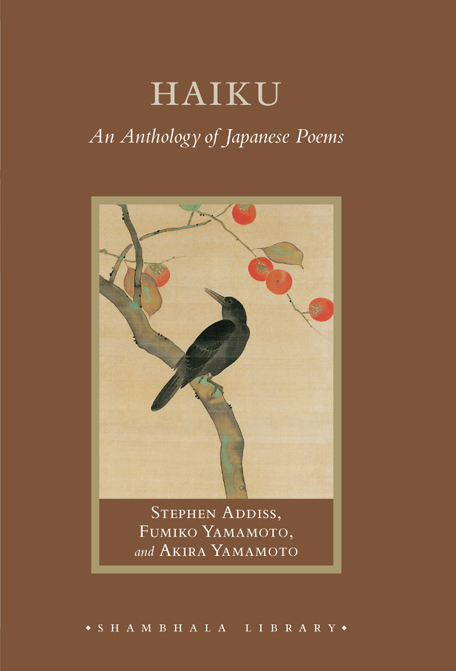
\includegraphics[width=\textwidth]{anthology}
\end{figure}

\chapter{Introduction}

\begin{figure}
    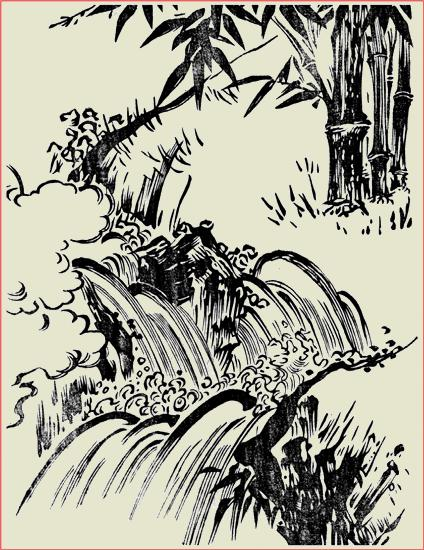
\includegraphics[width=\textwidth]{anthology-01}
\end{figure}

\setcounter{haikucounter}{0}

\begin{haiku}
    {\FH 夜の蘭香にかくれてや花白し}\hfill{\FH 蕪村}

    \vin{} Evening orchid---
    \vin{} \vin{} is it hidden in its scent?
    \vin{} \vin{} \vin{} the white of its flower

\end{haiku}

\begin{haiku}
    {\FH まよひ子のをの\ruby{か}{が}太鼓\ruby{て}{で}\ruby{尋}{たずね}られ}\hfill{\FH 無名氏}

    \vin{} The lost child
    \vin{} \vin{} with his own drum
    \vin{} \vin{} \vin{} is searched for
\end{haiku}

\chapter{The Pulse of Nature}

\begin{figure}
    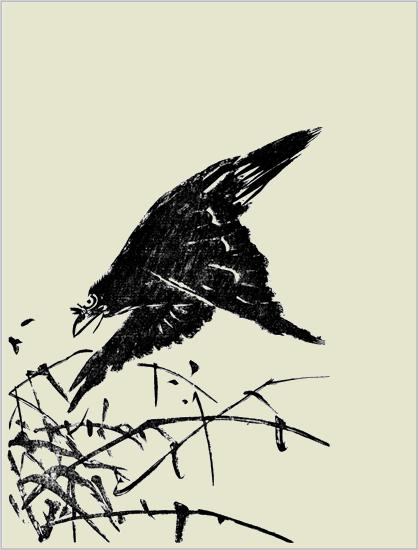
\includegraphics[width=\textwidth]{anthology-02}
\end{figure}

\begin{haiku}
    {\FH 打解けて氷と水の仲なほり}\hfill{\FH 貞室}

    \vin{} Opening their hearts
    \vin{} \vin{} ice and water become
    \vin{} \vin{} \vin{} friends again
    \hspace*{\fill} TEISHITSU
\end{haiku}

\begin{haiku}
    {\FH 春の日の\ruby{威光}{いこう}をみする雪間哉}\hfill{\FH 重頼}

    \vin{} The spring sun
    \vin{} \vin{} shows its power
    \vin{} \vin{} \vin{} between snowfalls \hspace{\fill} SHIGEYORI
\end{haiku}

\begin{haiku}
    {\FH ひたすらに咲うでもなし門の梅}\hfill{\FH 一茶}

    \vin{} Not in a hurry
    \vin{} \vin{} to blossom---
    \vin{} \vin{} \vin{} plum tree at my gate \hspace{\fill} ISSA
\end{haiku}

\begin{haiku}
    {\FH しら梅の枯木にもどる月夜哉}\hfill{\FH 蕪村}

    \vin{} White plum blossoms
    \vin{} \vin{} return to the withered tree---
    \vin{} \vin{} \vin{} moonlit night \hspace{\fill} BUSON
\end{haiku}

\begin{haiku}
    {\FH 鶯や泥足ぬぐふ梅の花}\hfill{\FH 一茶}

    \vin{} The warbler
    \vin{} \vin{} wipes its muddy feet
    \vin{} \vin{} \vin{} on plum blossoms \hspace{\fill} ISSA
\end{haiku}

\begin{haiku}
    {\FH 散るたびに老ゆく梅の木末かな}\hfill{\FH 蕪村}

    \vin{} With each falling petal
    \vin{} \vin{} they grow older---
    \vin{} \vin{} \vin{} plum branches \hspace{\fill} BUSON
\end{haiku}

\begin{haiku}
    {\FH 枯芝ややゝ\ruby{陽炎}{かげろふ}の一二寸}\hfill{\FH 芭蕉}

    \vin{} Dried grasses---
    \vin{} \vin{} and just a few heat waves
    \vin{} \vin{} \vin{} rising an inch or two \hspace{\fill} BASH\={O}
\end{haiku}

\begin{haiku}
    {\FH 愛あまる猫は傾婦の\ruby{媚}{こび}を仮る}\hfill{\FH 才麿}

    \vin{} Overflowing with love
    \vin{} \vin{} the cat as coquettish
    \vin{} \vin{} \vin{} as a courtesan \hspace{\fill} SAIMARO
\end{haiku}

\begin{haiku}
    {\FH 両方に髭があるなり猫の恋}\hfill{\FH 来山}

    \vin{} Both partners
    \vin{} \vin{} sport whiskers---
    \vin{} \vin{} \vin{} cats' love \hspace{\fill} RAIZAN
\end{haiku}

\begin{haiku}
    {\FH 春の日や水さへあれば暮残り}\hfill{\FH 一茶}

    \vin{} Spring sun
    \vin{} \vin{} in every pool of water---
    \vin{} \vin{} \vin{} lingering \hspace{\fill} ISSA
\end{haiku}

\begin{haiku}
    {\FH 曉も埋めたまゝや朧月}\hfill{\FH 鳥酔}

    \vin{} Is the dawn, too,
    \vin{} \vin{} still embraced by
    \vin{} \vin{} \vin{} hazy moon? \hspace{\fill} CH\={O}SUI
\end{haiku}

\begin{haiku}
    {\FH 陽炎に何やら猫の寝言哉}\hfill{\FH 一茶}

    \vin{} In the shimmering haze
    \vin{} \vin{} the cat mumbles something
    \vin{} \vin{} \vin{} in its sleep \hspace{\fill} ISSA
\end{haiku}

\begin{haiku}
    {\FH 春雨や小磯の小貝ぬるるほど}\hfill{\FH 蕪村}

    \vin{} Spring rain---
    \vin{} \vin{} just enough to wet tiny shells
    \vin{} \vin{} \vin{} on the tiny beach \hspace{\fill} BUSON
\end{haiku}

\begin{figure}
    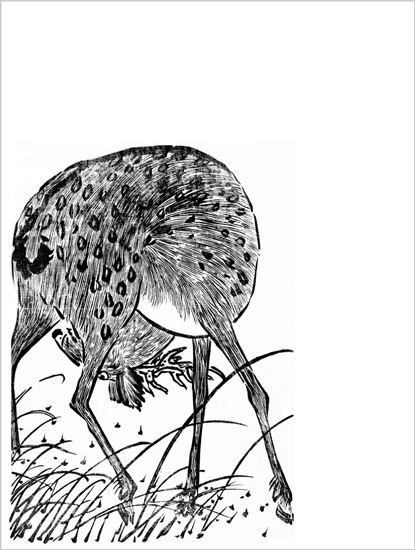
\includegraphics[width=\textwidth]{anthology-03}
\end{figure}

\begin{haiku}
    {\FH \ruby{植木}{うえき}屋のおいて行たる胡蝶かな}\hfill{\FH 蓼太}

    \vin{} The nurseryman
    \vin{} \vin{} left behind
    \vin{} \vin{} \vin{} a butterfly \hspace{\fill} RY\={O}TA
\end{haiku}

\begin{haiku}
    {\FH くりかへし麦の\ruby{畝}{うね}ぬふ小蝶かな}\hfill{\FH 曾良}

    \vin{} Again and again
    \vin{} \vin{} stitching the rows of barley---
    \vin{} \vin{} \vin{} a butterfly \hspace{\fill} SORA
\end{haiku}

\begin{haiku}
    {\FH 雉の尾のやさしくさはる菫かな}\hfill{\FH 秋色女}

    \vin{} A pheasant's tail
    \vin{} \vin{} very gently brushes
    \vin{} \vin{} \vin{} the violets \hspace{\fill} SH\={U}SHIKI-JO
\end{haiku}

\begin{haiku}
    {\FH 菫越して小さき風の渡りけり}\hfill{\FH 温亭}

    \vin{} Over the violets
    \vin{} \vin{} a small breeze
    \vin{} \vin{} \vin{} passes by \hspace{\fill} ONTEI
\end{haiku}

\begin{haiku}
    {\FH 吹くたびに蝶のゐなほる柳かな}\hfill{\FH 芭蕉}

    \vin{} Each time the wind blows
    \vin{} \vin{} the butterfly sits anew
    \vin{} \vin{} \vin{} on the willow \hspace{\fill} BASH\={O}
\end{haiku}

\begin{haiku}
    {\FH 春寒し水田の上の根さし雲}\hfill{\FH 碧梧桐}

    \vin{} Spring chill---
    \vin{} \vin{} above the rice paddies
    \vin{} \vin{} \vin{} rootless clouds \hspace{\fill} HEKIGOD\={O}
\end{haiku}

\begin{haiku}
    {\FH あけぼのや白魚白きこと一寸}\hfill{\FH 芭蕉}

    \vin{} Daybreak---
    \vin{} \vin{} the whitefish whiten
    \vin{} \vin{} \vin{} only one inch \hspace{\fill} BASH\={O}
\end{haiku}

\begin{haiku}
    NOT FOUND\hfill{---}

    \vin{} Domestic ducks
    \vin{} \vin{} stretch their necks
    \vin{} \vin{} \vin{} hoping to see the world \hspace{\fill} K\={O}JI
\end{haiku}

\begin{haiku}
    {\FH 鶯の笠\ruby{落}{おと}したる椿かな}\hfill{\FH 芭蕉}

    \vin{} The warbler
    \vin{} \vin{} dropped his hat---
    \vin{} \vin{} \vin{} a camellia \hspace{\fill} BASH\={O}
\end{haiku}

\begin{haiku}
    {\FH 花に狂ひ月に驚く胡蝶かな}\hfill{\FH 樗良}

    \vin{} Crazed by flowers
    \vin{} \vin{} surprised by the moon---
    \vin{} \vin{} \vin{} a butterfly \hspace{\fill} CHORA
\end{haiku}

\begin{haiku}
    {\FH 白椿落つる音のみ月夜かな}\hfill{\FH 闌更}

    \vin{} White camellias---
    \vin{} \vin{} only the sound of their falling
    \vin{} \vin{} \vin{} moonlit night \hspace{\fill} RANK\={O}
\end{haiku}

\begin{haiku}
    {\FH 雀子と声鳴きかはす鼠の巣}\hfill{\FH 芭蕉}

    \vin{} Squeaking in response
    \vin{} \vin{} to baby sparrows---
    \vin{} \vin{} \vin{} a nest of mice \hspace{\fill} BASH\={O}
\end{haiku}

\begin{figure}
    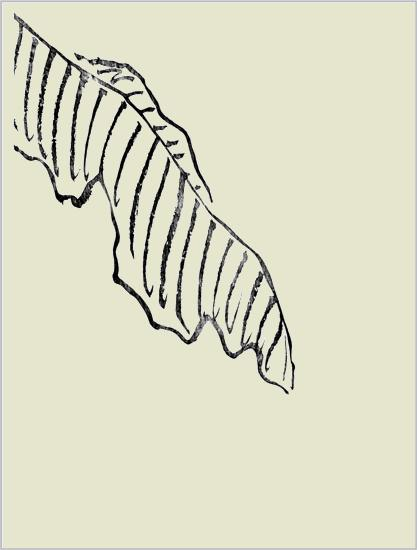
\includegraphics[width=\textwidth]{anthology-04}
\end{figure}

\begin{haiku}
    {\FH \ruby{闇}{くらき}より闇に入るや猫の恋}\hfill{\FH 一茶}

    \vin{} Out from the darkness
    \vin{} \vin{} back into the darkness---
    \vin{} \vin{} \vin{} affairs of the cat \hspace{\fill} ISSA
\end{haiku}

\begin{haiku}
    {\FH 夜はうれしく昼は静なり春の雨}\hfill{\FH 樗良}

    \vin{} Joyful at night
    \vin{} \vin{} tranquil during the day---
    \vin{} \vin{} \vin{} spring rain \hspace{\fill} CHORA
\end{haiku}

\begin{haiku}
    {\FH 椿落て昨日の雨をこぼしけり}\hfill{\FH 蕪村}

    \vin{} A camellia falls
    \vin{} \vin{} spilling out
    \vin{} \vin{} \vin{} yesterday's rain \hspace{\fill} BUSON
\end{haiku}

\begin{haiku}
    {\FH 茨\ruby{垣}{かき}犬の上手に\ruby{潜}{くぐ}りけり}\hfill{\FH 一茶}

    \vin{} A hedge of thorns---
    \vin{} \vin{} how skillfully the dog
    \vin{} \vin{} \vin{} wriggled under it! \hspace{\fill} ISSA
\end{haiku}

\begin{haiku}
    {\FH かすむ日の咄するやらのべの馬}\hfill{\FH 一茶}

    \vin{} Misty day---
    \vin{} \vin{} they might be gossiping
    \vin{} \vin{} \vin{} horses in the field \hspace{\fill} ISSA
\end{haiku}

\begin{haiku}
    {\FH 古井戸の暗きに落る椿かな}\hfill{\FH 蕪村}

    \vin{} An old well---
    \vin{} \vin{} falling into its darkness
    \vin{} \vin{} \vin{} a camellia \hspace{\fill} BUSON
\end{haiku}

\begin{haiku}
    {\FH 雲をふみ霞を吸うやあげ雲雀}\hfill{\FH 子規}

    \vin{} Trampling on clouds,
    \vin{} \vin{} inhaling the mist,
    \vin{} \vin{} \vin{} the skylark soars \hspace{\fill} SHIKI
\end{haiku}

\begin{haiku}
    {\FH \ruby{踞}{うずく}\ruby{ふ}{ば}て雲を\ruby{伺}{うかが}ふ蛙かな}\hfill{\FH 千代女}

    \vin{} Crouching,
    \vin{} \vin{} studying the clouds---
    \vin{} \vin{} \vin{} a frog \hspace{\fill} CHIYO-JO
\end{haiku}

\begin{haiku}
    {\FH 釣鐘にとまりて眠る胡蝶かな}\hfill{\FH 蕪村}

    \vin{} On the temple bell
    \vin{} \vin{} perching and sleeping---
    \vin{} \vin{} \vin{} a butterfly \hspace{\fill} BUSON
\end{haiku}

\begin{haiku}
    {\FH \ruby{釋教}{しゃっきょう}の歌か寺井に鳴くかへる}\hfill{\FH 閑節}

    \vin{} Could they be sutras?
    \vin{} \vin{} in the temple well
    \vin{} \vin{} \vin{} frogs chant \hspace{\fill} KANSETSU
\end{haiku}

\begin{haiku}
    {\FH 長く鳴く蛙の歌や文字\ruby{余}{あま}り}\hfill{\FH 永治}

    \vin{} Recited on and on,
    \vin{} \vin{} the poems of the frogs
    \vin{} \vin{} \vin{} have too many syllables \hspace{\fill} EIJI
\end{haiku}

\begin{haiku}
    {\FH 手をついて歌申しあぐる蛙かな}\hfill{\FH 宗鑑}

    \vin{} Bracing his feet
    \vin{} \vin{} and offering up a song---
    \vin{} \vin{} \vin{} the frog \hspace{\fill} S\={O}KAN
\end{haiku}

\begin{haiku}
    {\FH 大仏の鼻から出たる\ruby{乙鳥}{つばめ}哉}\hfill{\FH 一茶}

    \vin{} From the nostril
    \vin{} \vin{} of the Great Buddha comes
    \vin{} \vin{} \vin{} a swallow \hspace{\fill} ISSA
\end{haiku}

\begin{figure}
    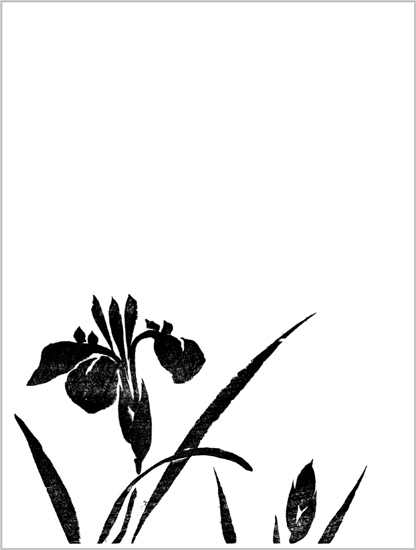
\includegraphics[width=\textwidth]{anthology-05}
\end{figure}

\begin{haiku}
    {\FH \ruby{柴門}{しばのと}や錠のかはりのかたつぶり}\hfill{\FH 一茶}

    \vin{} On the brushwood gate
    \vin{} \vin{} in place of a lock---
    \vin{} \vin{} \vin{} one snail \hspace{\fill} ISSA
\end{haiku}

\begin{haiku}
    {\FH 日の影や眠れる蝶に\ruby{透}{す}き通り}\hfill{\FH 闌更}

    \vin{} Sunlight
    \vin{} \vin{} passes through a butterfly
    \vin{} \vin{} \vin{} asleep \hspace{\fill} RANK\={O}
\end{haiku}

\begin{haiku}
    {\FH 取りつかぬ心で\ruby{浮}{う}かむ蛙かな}\hfill{\FH 丈草}

    \vin{} With the power of non-attachment
    \vin{} \vin{} floating on the water---
    \vin{} \vin{} \vin{} a frog \hspace{\fill} J\={O}S\={O}
\end{haiku}

\begin{haiku}
    {\FH 花を照らし月また花にくもる哉}\hfill{\FH 樗良}

    \vin{} Highlighting the blossoms,
    \vin{} \vin{} clouded by blossoms---
    \vin{} \vin{} \vin{} the moon \hspace{\fill} CHORA
\end{haiku}

\begin{haiku}
    {\FH 花びらの山を動かす桜かな}\hfill{\FH 抱一}

    \vin{} Flower petals
    \vin{} \vin{} set the mountain in motion---
    \vin{} \vin{} \vin{} cherry blossoms \hspace{\fill} H\={O}ITSU
\end{haiku}

\begin{haiku}
    {\FH 一めんの\ruby{落花}{らっか}の水に蛙の眼}\hfill{\FH 風生}

    \vin{} On the surface
    \vin{} \vin{} of petal-covered water---
    \vin{} \vin{} \vin{} frogs' eyes \hspace{\fill} F\={U}SEI
\end{haiku}

\begin{haiku}
    {\FH 行く春のうしろ姿や藤の花}\hfill{\FH 可南女}

    \vin{} The retreating shapes
    \vin{} \vin{} of the passing spring---
    \vin{} \vin{} \vin{} wisteria \hspace{\fill} KANA-JO
\end{haiku}

\begin{haiku}
    {\FH 行春や\ruby{逡}{しゆん}\ruby{巡}{じゆん}として遅ざくら}\hfill{\FH 蕪村}

    \vin{} Spring passes---
    \vin{} \vin{} the last reluctant
    \vin{} \vin{} \vin{} cherry blossoms \hspace{\fill} BUSON
\end{haiku}

\begin{figure}
    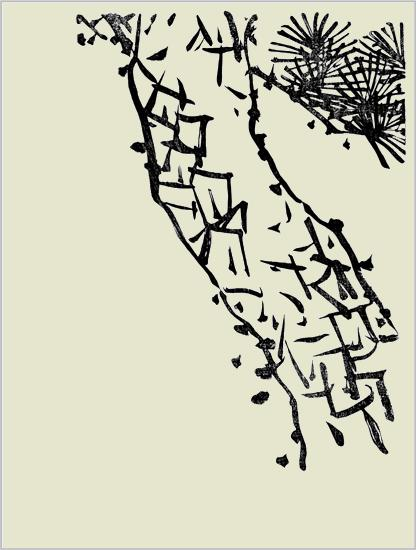
\includegraphics[width=\textwidth]{anthology-06}
\end{figure}

\begin{haiku}
    {\FH 浅河の西し東シす若葉哉}\hfill{\FH 蕪村}

    \vin{} Shallow river
    \vin{} \vin{} twisting west and twisting east---
    \vin{} \vin{} \vin{} young leaves \hspace{\fill} BUSON
\end{haiku}

\begin{haiku}
    {\FH \ruby{連翹}{れんぎょう}のまぶしき春の\ruby{憂}{うれ}ひかな}\hfill{\FH 万太郎}

    \vin{} Forsythia---
    \vin{} \vin{} and radiant spring's
    \vin{} \vin{} \vin{} melancholy \hspace{\fill} MANTAR\={O}
\end{haiku}

\begin{haiku}
    {\FH 日は日くれよ夜は夜明ケよと啼蛙}\hfill{\FH 蕪村}

    \vin{} In daytime ``darken the day''
    \vin{} \vin{} at night ``brighten the night''
    \vin{} \vin{} \vin{} frogs chant \hspace{\fill} BUSON
\end{haiku}

\begin{haiku}
    {\FH 海越て霞の網に入日哉}\hfill{\FH 蕪村}

    \vin{} Crossing the sea
    \vin{} \vin{} into a net of mist---
    \vin{} \vin{} \vin{} the setting sun \hspace{\fill} BUSON
\end{haiku}

\begin{haiku}
    {\FH 草霞み水に声なき日ぐれ哉}\hfill{\FH 蕪村}

    \vin{} Misty grasses---
    \vin{} \vin{} water without voices
    \vin{} \vin{} \vin{} in the dusk \hspace{\fill} BUSON
\end{haiku}

\begin{haiku}
    {\FH 行く春や海を見て居る鴉の子}\hfill{\FH 諸九}

    \vin{} Spring passing---
    \vin{} \vin{} looking at the sea,
    \vin{} \vin{} \vin{} a baby crow \hspace{\fill} SHOKY\={U}
\end{haiku}

\begin{haiku}
    {\FH \ruby{郭公}{ほととぎす}一声夏をさだめけり}\hfill{\FH 蓼太}

    \vin{} The cuckoo
    \vin{} \vin{} with a single song
    \vin{} \vin{} \vin{} has established summer \hspace{\fill} RY\={O}TA
\end{haiku}

\begin{haiku}
    {\FH ほととぎす声や横たふ水の上}\hfill{\FH 芭蕉}

    \vin{} The voice of the cuckoo
    \vin{} \vin{} slants
    \vin{} \vin{} \vin{} over the water \hspace{\fill} BASH\={O}
\end{haiku}

\begin{haiku}
    {\FH 郭公鳴くや湖水のささにごり}\hfill{\FH 丈草}

    \vin{} The cuckoo calls---
    \vin{} \vin{} and the waters of the lake
    \vin{} \vin{} \vin{} cloud over a little \hspace{\fill} J\={O}S\={O}
\end{haiku}

\begin{haiku}
    {\FH 時鳥蝿虫めらもよっく聞け}\hfill{\FH 一茶}

    \vin{} The cuckoo---
    \vin{} \vin{} flies and insects,
    \vin{} \vin{} \vin{} listen well! \hspace{\fill} ISSA
\end{haiku}

\begin{haiku}
    {\FH 五月雨や梅の葉寒き風の色}\hfill{\FH 才麿}

    \vin{} Summer rains---
    \vin{} \vin{} leaves of the plum
    \vin{} \vin{} \vin{} the color of cold wind \hspace{\fill} SAIMARO
\end{haiku}

\begin{haiku}
    {\FH 五月雨や滄海を衝く濁水}\hfill{\FH 蕪村}

    \vin{} Early summer rains---
    \vin{} \vin{} lunging at the blue sea
    \vin{} \vin{} \vin{} muddy waters \hspace{\fill} BUSON
\end{haiku}

\begin{figure}
    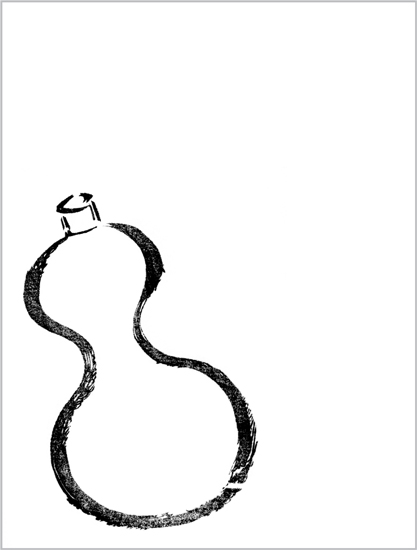
\includegraphics[width=\textwidth]{anthology-07}
\end{figure}

\begin{haiku}
    {\FH 五月雨の名もなき川のおそろしき}\hfill{\FH 蕪村}

    \vin{} Early summer rains---
    \vin{} \vin{} even nameless rivers
    \vin{} \vin{} \vin{} are fearsome \hspace{\fill} BUSON
\end{haiku}

\begin{haiku}
    {\FH 涼しさや青田の中の一つ松}\hfill{\FH 子規}

    \vin{} Summer cool---
    \vin{} \vin{} in the green rice fields
    \vin{} \vin{} \vin{} a single pine \hspace{\fill} SHIKI
\end{haiku}

\begin{haiku}
    {\FH 不二ひとつ埋み残して若葉かな}\hfill{\FH 蕪村}

    \vin{} Only Fuji
    \vin{} \vin{} remains unburied---
    \vin{} \vin{} \vin{} young leaves \hspace{\fill} BUSON
\end{haiku}

\begin{haiku}
    {\FH 紫陽花におもたき朝日夕日哉}\hfill{\FH 乙由}

    \vin{} On the hydrangeas
    \vin{} \vin{} the weight of the morning sun,
    \vin{} \vin{} \vin{} the evening sun \hspace{\fill} OTSUY\={U}
\end{haiku}

\begin{haiku}
    {\FH 山蟻のあからさま也白牡丹}\hfill{\FH 蕪村}

    \vin{} Mountain ant---
    \vin{} \vin{} seen so clearly
    \vin{} \vin{} \vin{} on the white peony \hspace{\fill} BUSON
\end{haiku}

\begin{haiku}
    {\FH ひとりひつそり竹の子竹になる}\hfill{\FH 山頭火}

    \vin{} Alone, silently---
    \vin{} \vin{} the bamboo shoot
    \vin{} \vin{} \vin{} becomes a bamboo \hspace{\fill} SANT\={O}KA
\end{haiku}

\begin{haiku}
    {\FH 鶯や竹の子薮に老を鳴く}\hfill{\FH 芭蕉}

    \vin{} The warbler
    \vin{} \vin{} amid the bamboo shoots
    \vin{} \vin{} \vin{} sings of old age \hspace{\fill} BASH\={O}
\end{haiku}

\begin{haiku}
    {\FH 三角のいとま\ruby{蜥蜴}{とかげ}の顔の少し延ぶか}\hfill{\FH 虚子}

    \vin{} A triangle---
    \vin{} \vin{} is the lizard's head getting
    \vin{} \vin{} \vin{} a little longer? \hspace{\fill} KYOSHI
\end{haiku}

\begin{haiku}
    {\FH 我宿や鼠と仲のよい蛍}\hfill{\FH 一茶}

    \vin{} In my dwelling
    \vin{} \vin{} friendly with the mice---
    \vin{} \vin{} \vin{} fireflies \hspace{\fill} ISSA
\end{haiku}

\begin{haiku}
    {\FH おもしろや左右の使の飛ぶほたる}\hfill{\FH 介我}

    \vin{} How interesting---
    \vin{} \vin{} running errands right and left
    \vin{} \vin{} \vin{} fireflies \hspace{\fill} KAIGA
\end{haiku}

\begin{haiku}
    {\FH 追れては月にかくるるほたる哉}\hfill{\FH 蓼太}

    \vin{} Pursued,
    \vin{} \vin{} it hides in the moon---
    \vin{} \vin{} \vin{} the firefly \hspace{\fill} RY\={O}TA
\end{haiku}

\begin{haiku}
    {\FH もえやすく又消やすき蛍哉}\hfill{\FH 千子女}

    \vin{} Burning so easily,
    \vin{} \vin{} extinguishing so easily---
    \vin{} \vin{} \vin{} the firefly \hspace{\fill} CHINE-JO
\end{haiku}

\begin{haiku}
    {\FH 朝風に毛を\ruby{吹}{ふか}れ居る毛むし哉}\hfill{\FH 蕪村}

    \vin{} The morning breeze
    \vin{} \vin{} ripples the fur
    \vin{} \vin{} \vin{} of the caterpillar \hspace{\fill} BUSON
\end{haiku}

\begin{figure}
    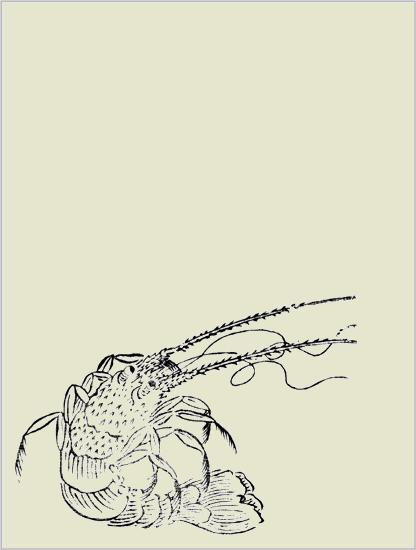
\includegraphics[width=\textwidth]{anthology-08}
\end{figure}

\begin{haiku}
    {\FH 湖に尻を吹かせて蝉の鳴}\hfill{\FH 一茶}

    \vin{} As the lake breeze
    \vin{} \vin{} cools his bottom
    \vin{} \vin{} \vin{} the cicada cries \hspace{\fill} ISSA
\end{haiku}

\begin{haiku}
    {\FH 稲妻につむりなでけり\ruby{引蟇}{ひきがえる}}\hfill{\FH 一茶}

    \vin{} As lightning flashes
    \vin{} \vin{} he strokes his head---
    \vin{} \vin{} \vin{} the toad \hspace{\fill} ISSA
\end{haiku}

\begin{haiku}
    {\FH 蛇逃げて我を見し眼の草に残る}\hfill{\FH 虚子}

    \vin{} The snake flees---
    \vin{} \vin{} but the eyes that peered at me
    \vin{} \vin{} \vin{} remain in the weeds \hspace{\fill} KYOSHI
\end{haiku}

\begin{haiku}
    {\FH さはさはと蓮うごかす池の亀}\hfill{\FH 鬼貫}

    \vin{} Rustling, rustling,
    \vin{} \vin{} the lotus leaves sway---
    \vin{} \vin{} \vin{} a tortoise in the pond \hspace{\fill} ONITSURA
\end{haiku}

\begin{haiku}
    {\FH けふの日も棒ふり虫よ翌も又}\hfill{\FH 一茶}

    \vin{} Today too
    \vin{} \vin{} mosquito larvae---
    \vin{} \vin{} \vin{} and tomorrow again \hspace{\fill} ISSA
\end{haiku}

\begin{haiku}
    NOT FOUND\hfill{\FH 無名氏}

    \vin{} As flies retreat
    \vin{} \vin{} mosquitoes start
    \vin{} \vin{} \vin{} their battle cry \hspace{\fill} ANONYMOUS
\end{haiku}

\begin{haiku}
    NOT FOUND\hfill{\FH 無名氏}

    \vin{} Dashing into one another
    \vin{} \vin{} whispering, parting---
    \vin{} \vin{} \vin{} ants \hspace{\fill} ANONYMOUS
\end{haiku}

\begin{haiku}
    {雲を吐き雲を吸い込む峰の松}\hfill{\FH 無名氏}

    \vin{} Inhaling clouds
    \vin{} \vin{} exhaling clouds---
    \vin{} \vin{} \vin{} mountaintop pines \hspace{\fill} ANONYMOUS
\end{haiku}

\begin{figure}
    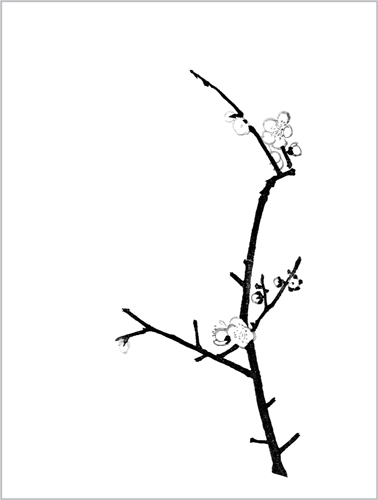
\includegraphics[width=\textwidth]{anthology-09}
\end{figure}

\begin{haiku}
    {\FH 蚊\ruby{柱}{ばしら}に夢の浮橋かかるなり}\hfill{\FH 其角}

    \vin{} Across a pillar of mosquitoes
    \vin{} \vin{} hangs the bridge
    \vin{} \vin{} \vin{} of dreams \hspace{\fill} KIKAKU
\end{haiku}

\begin{haiku}
    {\FH 蛤の口しめてゐる暑さかな}\hfill{\FH 芭蕉}

    \vin{} Even the clams
    \vin{} \vin{} keep their mouths shut
    \vin{} \vin{} \vin{} in this heat \hspace{\fill} BASH\={O}
\end{haiku}

\begin{haiku}
    {\FH 古壁の隅に動かずはらみ蜘}\hfill{\FH 子規}

    \vin{} Motionless
    \vin{} \vin{} in a crevice of an old wall---
    \vin{} \vin{} \vin{} a pregnant spider \hspace{\fill} SHIKI
\end{haiku}

\begin{haiku}
    {\FH \ruby{濤}{なみ}暑し石に\ruby{怒}{いか}れるひびきあり}\hfill{\FH 暁台}

    \vin{} Heat in waves---
    \vin{} \vin{} in the stones
    \vin{} \vin{} \vin{} angry reverberations \hspace{\fill} KY\={O}TAI
\end{haiku}

\begin{haiku}
    {\FH ゆふ立やよみがへりたる\ruby{斃}{たおれ}馬}\hfill{\FH 几董}

    \vin{} Sudden shower---
    \vin{} \vin{} and rising from the heat,
    \vin{} \vin{} \vin{} the broken-down horse \hspace{\fill} KIT\={O}
\end{haiku}

\begin{haiku}
   NOT FOUND\hfill{---}

    \vin{} Lightning!
    \vin{} \vin{} fleeing up the wall,
    \vin{} \vin{} \vin{} the legs of a spider \hspace{\fill} KICH\={O}
\end{haiku}

\begin{haiku}
    {\FH 夕立や草葉をつかむむら雀}\hfill{\FH 蕪村}

    \vin{} Sudden shower---
    \vin{} \vin{} clutching the blades of grass
    \vin{} \vin{} \vin{} a flock of sparrows \hspace{\fill} BUSON
\end{haiku}

\begin{haiku}
    {\FH 桐の木や雨のながるる蝉の腹}\hfill{\FH 梅室}

    \vin{} Down a paulownia tree
    \vin{} \vin{} the rain comes trickling
    \vin{} \vin{} \vin{} across a cicada's belly \hspace{\fill} BAISHITSU
\end{haiku}

\begin{haiku}
    {\FH \ruby{雨蛙}{あまがえる}芭蕉にのりてそよぎけり}\hfill{\FH 其角}

    \vin{} The tree frog
    \vin{} \vin{} riding the plantain leaf
    \vin{} \vin{} \vin{} sways \hspace{\fill} KIKAKU
\end{haiku}

\begin{haiku}
    {\FH ばか長い日やと口明く烏哉}\hfill{\FH 一茶}

    \vin{} ``It's much too long a day'',
    \vin{} \vin{} opening its mouth
    \vin{} \vin{} \vin{} a crow \hspace{\fill} ISSA
\end{haiku}

\begin{haiku}
    {\FH 魚どもは桶としらでや夕涼}\hfill{\FH 一茶}

    \vin{} The fish
    \vin{} \vin{} not knowing they're in a bucket
    \vin{} \vin{} \vin{} cool by the gate \hspace{\fill} ISSA
\end{haiku}

\begin{haiku}
    {\FH 夕立にうたるゝ鯉のかしらかな}\hfill{\FH 子規}

    \vin{} A sudden shower
    \vin{} \vin{} drums down upon
    \vin{} \vin{} \vin{} the heads of the carp \hspace{\fill} SHIKI
\end{haiku}

\begin{haiku}
    {\FH いなづまやきのふは東けふは西}\hfill{\FH 其角}

    \vin{} Lightning---
    \vin{} \vin{} yesterday to the east
    \vin{} \vin{} \vin{} today to the west \hspace{\fill} KIKAKU
\end{haiku}

\begin{haiku}
    {\FH 一本の草も涼風やどりけり}\hfill{\FH 一茶}

    \vin{} Even in a single blade of grass
    \vin{} \vin{} the cool breeze
    \vin{} \vin{} \vin{} finds a home \hspace{\fill} ISSA
\end{haiku}

\begin{haiku}
    {\FH 飛ぶ鮎の底に雲ゆく流かな}\hfill{\FH 鬼貫}

    \vin{} The trout leaps up---
    \vin{} \vin{} and below him in a stream
    \vin{} \vin{} \vin{} clouds float by \hspace{\fill} ONITSURA
\end{haiku}

\begin{haiku}
    {\FH しづかさや湖水の底の雲のみね}\hfill{\FH 一茶}

    \vin{} How quiet---
    \vin{} \vin{} at the bottom of the lake
    \vin{} \vin{} \vin{} peaks of clouds \hspace{\fill} ISSA
\end{haiku}

\begin{haiku}
    {\FH 海の音にひまわり黒き瞳をひらく}\hfill{\FH 夕爾}

    \vin{} At the sound of the sea
    \vin{} \vin{} the sunflowers open
    \vin{} \vin{} \vin{} their black eyes \hspace{\fill} Y\={U}JI
\end{haiku}

\begin{haiku}
    {\FH 蛸壺やはかなき夢を夏の月}\hfill{\FH 芭蕉}

    \vin{} Octopus pot---
    \vin{} \vin{} evanescent dreams
    \vin{} \vin{} \vin{} of the summer moon \hspace{\fill} BASH\={O}
\end{haiku}

\begin{haiku}
    {\FH 短夜や\ruby{芦}{あし}間流るる蟹の\ruby{泡}{あわ}}\hfill{\FH 蕪村}

    \vin{} Short summer night---
    \vin{} \vin{} flowing through reeds
    \vin{} \vin{} \vin{} bubbles from crabs \hspace{\fill} BUSON
\end{haiku}

\begin{haiku}
    {\FH 閑さや岩にしみ入る蝉の声}\hfill{\FH 芭蕉}

    \vin{} Stillness---
    \vin{} \vin{} seeping into the rocks
    \vin{} \vin{} \vin{} the cicada's voice \hspace{\fill} BASH\={O}
\end{haiku}

\begin{haiku}
    {\FH うつくしく牛の痩せたる夏野哉}\hfill{\FH 凡兆}

    \vin{} How beautifully
    \vin{} \vin{} the cow has slimmed down
    \vin{} \vin{} \vin{} in the summer fields \hspace{\fill} BONCH\={O}
\end{haiku}

\begin{haiku}
    {\FH 朝露や撫でて涼しき瓜の土}\hfill{\FH 芭蕉}

    \vin{} In the morning dew
    \vin{} \vin{} soiled and cooled---
    \vin{} \vin{} \vin{} dirt on the melon \hspace{\fill} BASH\={O}
\end{haiku}

\begin{figure}
    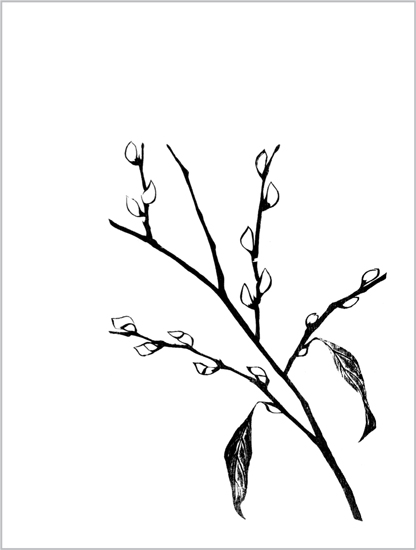
\includegraphics[width=\textwidth]{anthology-10}
\end{figure}

\begin{haiku}
    {\FH 涼しさや\ruby{行燈}{あん}どん消えて水の音}\hfill{\FH 子規}

    \vin{} Summer coolness---
    \vin{} \vin{} lantern out,
    \vin{} \vin{} \vin{} the sound of water \hspace{\fill} SHIKI
\end{haiku}

\begin{haiku}
    {\FH 五月雨やある夜ひそかに松の月}\hfill{\FH 蓼太}

    \vin{} Summer rains---
    \vin{} \vin{} secretly one evening
    \vin{} \vin{} \vin{} moon in the pines \hspace{\fill} RY\={O}TA
\end{haiku}

\begin{haiku}
    {\FH かはほりのかくれ住けり破れ傘}\hfill{\FH 蕪村}

    \vin{} The bat's
    \vin{} \vin{} secret home---
    \vin{} \vin{} \vin{} a tattered hat \hspace{\fill} BUSON
\end{haiku}

\begin{haiku}
    {\FH 夕顔の花\ruby{噛}{か}む猫や余所ごころ}\hfill{\FH 蕪村}

    \vin{} Evening glories---
    \vin{} \vin{} the cat chewing the flower
    \vin{} \vin{} \vin{} has its mind elsewhere \hspace{\fill} BUSON
\end{haiku}

\begin{haiku}
    {\FH 麦のほに尾を隠さばや老狐}\hfill{\FH 轍士}

    \vin{} Among the ears of barley
    \vin{} \vin{} are you hiding your tail?
    \vin{} \vin{} \vin{} old fox \hspace{\fill} TESSHI
\end{haiku}

\begin{haiku}
    {\FH 秋の季の赤とんぼうに\ruby{定}{さだ}まりぬ}\hfill{\FH 白雄}

    \vin{} The coming of autumn
    \vin{} \vin{} determined
    \vin{} \vin{} \vin{} by a red dragonfly \hspace{\fill} SHIRAO
\end{haiku}

\begin{haiku}
    {\FH 星既に秋の眼をひらきけり}\hfill{\FH 紅葉}

    \vin{} The stars
    \vin{} \vin{} have already opened
    \vin{} \vin{} \vin{} their autumn eyes \hspace{\fill} K\={O}Y\={O}
\end{haiku}

\begin{haiku}
    {\FH 初秋や夕立長引く夜の雨}\hfill{\FH 太祇}

    \vin{} Early autumn---
    \vin{} \vin{} the evening shower becomes
    \vin{} \vin{} \vin{} a night of rain \hspace{\fill} TAIGI
\end{haiku}

\begin{haiku}
    {\FH 初秋や海も青田も一みどり}\hfill{\FH 芭蕉}

    \vin{} Autumn begins---
    \vin{} \vin{} ocean and fields
    \vin{} \vin{} \vin{} all one green \hspace{\fill} BASH\={O}
\end{haiku}

\begin{haiku}
    {\FH はや秋の柳をすかす朝日かな}\hfill{\FH 成美}

    \vin{} Early autumn---
    \vin{} \vin{} peering through willows
    \vin{} \vin{} \vin{} the morning sun \hspace{\fill} SEIBI
\end{haiku}

\begin{haiku}
    {\FH 朝顔や吹倒されたなりに咲}\hfill{\FH 一茶}

    \vin{} Morning glories---
    \vin{} \vin{} blown to the ground
    \vin{} \vin{} \vin{} bloom as they are \hspace{\fill} ISSA
\end{haiku}

\begin{haiku}
    {\FH 露ほろりほろと鳩の念仏哉}\hfill{\FH 一茶}

    \vin{} As dew drips
    \vin{} \vin{} gently, gently, the dove
    \vin{} \vin{} \vin{} murmurs its chant \hspace{\fill} ISSA
\end{haiku}

\begin{haiku}
    {\FH 草も木も月待つ露の夕かな}\hfill{\FH 宗祇}

    \vin{} Grasses and trees all
    \vin{} \vin{} waiting for the moon---
    \vin{} \vin{} \vin{} dewy evening \hspace{\fill} S\={O}GI
\end{haiku}

\begin{figure}
    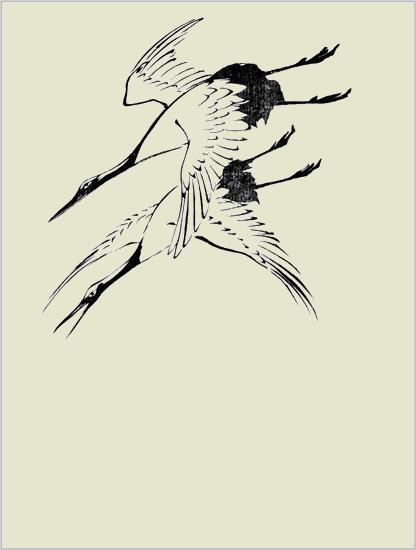
\includegraphics[width=\textwidth]{anthology-11}
\end{figure}

\begin{haiku}
    {\FH 白露や茨のとげにひとつずつ}\hfill{\FH 蕪村}

    \vin{} White dew
    \vin{} \vin{} on brambles and thorns---
    \vin{} \vin{} \vin{} one drop each \hspace{\fill} BUSON
\end{haiku}

\begin{haiku}
    {\FH \ruby{艸}{くさ}の葉を遊びありけよ露の玉}\hfill{\FH 嵐雪}

    \vin{} On blades of grass
    \vin{} \vin{} frolic and roll on---
    \vin{} \vin{} \vin{} pearls of dew \hspace{\fill} RANSETSU
\end{haiku}

\begin{haiku}
    {\FH 露凉し形あるもの皆生ける}\hfill{\FH 鬼城}

    \vin{} Dew cooling---
    \vin{} \vin{} things with shapes
    \vin{} \vin{} \vin{} all alive \hspace{\fill} KIJ\={O}
\end{haiku}

\begin{haiku}
    NOT FOUND\hfill{\FH 無名氏}

    \vin{} Its face
    \vin{} \vin{} looks like a horse---
    \vin{} \vin{} \vin{} the grasshopper \hspace{\fill} ANONYMOUS
\end{haiku}

\begin{haiku}
    {\FH 石にとんぼはまひるのゆめみる}\hfill{\FH 山頭火}

    \vin{} Dragonfly on a rock
    \vin{} \vin{} absorbed in
    \vin{} \vin{} \vin{} a daydream \hspace{\fill} SANT\={O}KA
\end{haiku}

\begin{haiku}
    {\FH 蜻蜒や取りつきかねし草の上}\hfill{\FH 芭蕉}

    \vin{} The dragonfly
    \vin{} \vin{} cannot come to rest
    \vin{} \vin{} \vin{} on the blades of grass \hspace{\fill} BASH\={O}
\end{haiku}

\begin{haiku}
    {\FH 猫の子のかくれんぼする萩の花}\hfill{\FH 一茶}

    \vin{} Kittens
    \vin{} \vin{} playing hide-and-seek
    \vin{} \vin{} \vin{} in the bush clover \hspace{\fill} ISSA
\end{haiku}

\begin{haiku}
    {\FH 蜻蛉やくるひ静まる三日の月}\hfill{\FH 其角}

    \vin{} Dragonflies
    \vin{} \vin{} quiet their mad darting---
    \vin{} \vin{} \vin{} crescent moon \hspace{\fill} KIKAKU
\end{haiku}

\begin{figure}
    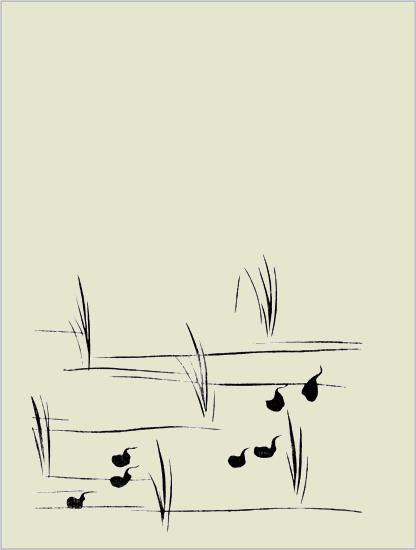
\includegraphics[width=\textwidth]{anthology-12}
\end{figure}

\begin{haiku}
    {\FH かはほりや月のあたりを立ちさらず}\hfill{\FH 暁台}

    \vin{} The bat
    \vin{} \vin{} circling the moon
    \vin{} \vin{} \vin{} would not leave it \hspace{\fill} KY\={O}TAI
\end{haiku}

\begin{haiku}
    {\FH 夢返せ烏の\ruby{覚}{さま}す霧の月}\hfill{\FH 鬼貫}

    \vin{} Give me back my dream!
    \vin{} \vin{} a crow has wakened me
    \vin{} \vin{} \vin{} to misty moonlight \hspace{\fill} ONITSURA
\end{haiku}

\begin{haiku}
    {\FH おのがみに秋を染め抜く蜻蛉かな}\hfill{\FH 麦水}

    \vin{} Dyeing his body
    \vin{} \vin{} autumn---
    \vin{} \vin{} \vin{} the dragonfly \hspace{\fill} BAKUSUI
\end{haiku}

\begin{haiku}
    {\FH 遠山が目玉にうつるとんぼかな}\hfill{\FH 一茶}

    \vin{} Distant mountains
    \vin{} \vin{} reflecting in its eyes---
    \vin{} \vin{} \vin{} a dragonfly \hspace{\fill} ISSA
\end{haiku}

\begin{haiku}
    NOT FOUND\hfill{\FH 無名氏}

    \vin{} A floating sandal---
    \vin{} \vin{} an object of scorn
    \vin{} \vin{} \vin{} to the plovers \hspace{\fill} ANONYMOUS
\end{haiku}

\begin{haiku}
    {\FH 松風や軒をめぐって秋暮れぬ }\hfill{\FH 芭蕉}

    \vin{} The pine wind
    \vin{} \vin{} circling around the eaves---
    \vin{} \vin{} \vin{} autumn deepens \hspace{\fill} BASH\={O}
\end{haiku}

\begin{haiku}
    {\FH 涼風や虚空にみちて松の声}\hfill{\FH 鬼貫}

    \vin{} Cool breeze
    \vin{} \vin{} filling the empty sky---
    \vin{} \vin{} \vin{} pine voices \hspace{\fill} ONITSURA
\end{haiku}

\begin{haiku}
    {\FH 山のしづかさへしづかなる雨}\hfill{\FH 山頭火}

    \vin{} To the mountain quietude
    \vin{} \vin{} the quiet
    \vin{} \vin{} \vin{} rain \hspace{\fill} SANT\={O}KA
\end{haiku}

\begin{haiku}
    {\FH 古犬が先に立也はか参り}\hfill{\FH 一茶}

    \vin{} The old dog
    \vin{} \vin{} is leading the way---
    \vin{} \vin{} \vin{} visiting family graves \hspace{\fill} ISSA
\end{haiku}

\begin{haiku}
    {\FH 野分やんで鼠のわたる流かな}\hfill{\FH 蕪村}

    \vin{} Typhoons ended,
    \vin{} \vin{} the rat swims across
    \vin{} \vin{} \vin{} flowing waters \hspace{\fill} BUSON
\end{haiku}

\begin{haiku}
    {\FH \ruby{三度}{みたび}啼て聞えずなりぬ鹿の声}\hfill{\FH 蕪村}

    \vin{} Calling three times,
    \vin{} \vin{} then no more to be heard---
    \vin{} \vin{} \vin{} the deer in the rain \hspace{\fill} BUSON
\end{haiku}

\begin{haiku}
    NOT FOUND\hfill{\FH 高政}

    \vin{} Running across the shelf
    \vin{} \vin{} hoisting a chrysanthemum---
    \vin{} \vin{} \vin{} a temple mouse \hspace{\fill} TAKAMASA
\end{haiku}

\begin{haiku}
   NOT FOUND\hfill{---}

    \vin{} On a withered branch
    \vin{} \vin{} lingers the evanescent memory
    \vin{} \vin{} \vin{} of a cicada's voice \hspace{\fill} KAGAI
\end{haiku}

\begin{haiku}
    {\FH 鳴ながら虫の流るる浮木かな}\hfill{\FH 一茶}

    \vin{} Singing as it goes,
    \vin{} \vin{} an insect floats down the stream
    \vin{} \vin{} \vin{} on a broken bough \hspace{\fill} ISSA
\end{haiku}

\begin{haiku}
    {\FH 鷹の目も今や暮れぬと鳴く鶉}\hfill{\FH 芭蕉}

    \vin{} ``The eyes of the hawks
    \vin{} \vin{} are now dimmed'',
    \vin{} \vin{} \vin{} quails sing \hspace{\fill} BASH\={O}
\end{haiku}

\begin{haiku}
    {\FH きりきりす鳴や案山子の袖の内}\hfill{\FH 智月}

    \vin{} A grasshopper
    \vin{} \vin{} chirps in the sleeve
    \vin{} \vin{} \vin{} of the scarecrow \hspace{\fill} CHIGETSU
\end{haiku}

\begin{haiku}
    {\FH 野は枯てのばす物なし鶴の首}\hfill{\FH 支考}

    \vin{} The fields have withered---
    \vin{} \vin{} no need for the crane
    \vin{} \vin{} \vin{} to stretch out its neck \hspace{\fill} SHIK\={O}
\end{haiku}

\begin{haiku}
    {\FH 初雁のおのが空問う夕暮れや}\hfill{\FH 士朗}

    \vin{} The first goose
    \vin{} \vin{} seeking its own sky
    \vin{} \vin{} \vin{} in the dusk \hspace{\fill} SHIR\={O}
\end{haiku}

\begin{haiku}
    {\FH 倒るれば倒るるままの庭の草}\hfill{\FH 良寛}

    \vin{} When they fall,
    \vin{} \vin{} just as they fall---
    \vin{} \vin{} \vin{} garden grasses \hspace{\fill} RY\={O}KAN
\end{haiku}

\begin{haiku}
    {\FH 山暮れて紅葉の朱を奪ひけり}\hfill{\FH 蕪村}

    \vin{} Mountains darken---
    \vin{} \vin{} robbing the scarlet
    \vin{} \vin{} \vin{} from maple leaves \hspace{\fill} BUSON
\end{haiku}

\begin{haiku}
    {\FH 月はやし梢は雨を持ちながら}\hfill{\FH 芭蕉}

    \vin{} The moon speeds on---
    \vin{} \vin{} the treetops
    \vin{} \vin{} \vin{} still holding rain \hspace{\fill} BASH\={O}
\end{haiku}

\begin{haiku}
    {\FH \ruby{巌}{いわ}月に\ruby{大坐}{おおま}する}\hfill{\FH 井泉水}

    \vin{} A rock
    \vin{} \vin{} against the moon
    \vin{} \vin{} \vin{} sits big \hspace{\fill} SEISENSUI
\end{haiku}

\begin{haiku}
    {\FH 名月や山のかがしの袂から}\hfill{\FH 一茶}

    \vin{} The bright moon---
    \vin{} \vin{} out from the sleeve
    \vin{} \vin{} \vin{} of the scarecrow \hspace{\fill} ISSA
\end{haiku}

\begin{haiku}
    {\FH 落葉おちかさなりて雨雨をうつ}\hfill{\FH 暁台}

    \vin{} Fallen leaves
    \vin{} \vin{} fall on each other---
    \vin{} \vin{} \vin{} rain beats on the rain \hspace{\fill} KY\={O}TAI
\end{haiku}

\begin{haiku}
    {\FH 西吹けば東にたまる落ち葉かな}\hfill{\FH 蕪村}

    \vin{} Blown from the west
    \vin{} \vin{} collecting in the east---
    \vin{} \vin{} \vin{} falling leaves \hspace{\fill} BUSON
\end{haiku}

\begin{haiku}
    {\FH 古池の蛙老ゆく落葉哉}\hfill{\FH 蕪村}

    \vin{} The old pond's
    \vin{} \vin{} frog also growing old---
    \vin{} \vin{} \vin{} fallen leaves \hspace{\fill} BUSON
\end{haiku}

\begin{haiku}
    {\FH 掃けるが終には掃ず落葉かな}\hfill{\FH 太祇}

    \vin{} Sweeping
    \vin{} \vin{} and then not sweeping
    \vin{} \vin{} \vin{} the fallen leaves \hspace{\fill} TAIGI
\end{haiku}

\begin{haiku}
    {\FH どっしりと尻を\ruby{据}{す}えたる\ruby{南瓜}{なんか}かな}\hfill{\FH 漱石}

    \vin{} Very squarely
    \vin{} \vin{} setting its buttocks down---
    \vin{} \vin{} \vin{} the pumpkin \hspace{\fill} S\={O}SEKI
\end{haiku}

\begin{haiku}
    {\FH 秋風の姿なりけりむらすすき}\hfill{\FH 季吟}

    \vin{} The autumn wind
    \vin{} \vin{} takes the shape
    \vin{} \vin{} \vin{} of pampas grass \hspace{\fill} KIGIN
\end{haiku}

\begin{haiku}
    {\FH 行秋の草にかくるゝ流かな}\hfill{\FH 白雄}

    \vin{} To passing autumn
    \vin{} \vin{} the pampas grass waves
    \vin{} \vin{} \vin{} goodbye goodbye \hspace{\fill} SHIRAO
\end{haiku}

\begin{haiku}
    {\FH 秋雨や蜘蛛とぢて伏す枯れ葎}\hfill{\FH 石鼎}

    \vin{} Autumn rains---
    \vin{} \vin{} a spider encased in
    \vin{} \vin{} \vin{} a clump of fallen grass \hspace{\fill} SEKITEI
\end{haiku}

\begin{haiku}
    {\FH 夕霧や馬の\ruby{覚}{おぼえ}し橋の穴}\hfill{\FH 一茶}

    \vin{} Evening fog---
    \vin{} \vin{} my horse has learned
    \vin{} \vin{} \vin{} the holes on the bridge \hspace{\fill} ISSA
\end{haiku}

\begin{haiku}
    {\FH 雨だれの音も年とった}\hfill{\FH 山頭火}

    \vin{} The sound
    \vin{} \vin{} of the raindrops
    \vin{} \vin{} \vin{} also grown older \hspace{\fill} SANT\={O}KA
\end{haiku}

\begin{haiku}
    {\FH 名月にけろりと立しかがし哉}\hfill{\FH 一茶}

    \vin{} In the harvest moonlight
    \vin{} \vin{} standing nonchalantly---
    \vin{} \vin{} \vin{} the scarecrow \hspace{\fill} ISSA
\end{haiku}

\begin{haiku}
    {\FH 笠とれて面目もなきかがしかな}\hfill{\FH 蕪村}

    \vin{} Its hat fallen off
    \vin{} \vin{} and embarrassed---
    \vin{} \vin{} \vin{} the scarecrow \hspace{\fill} BUSON
\end{haiku}

\begin{haiku}
    {\FH 朱を注ぐ入り日のあとは秋の暮}\hfill{\FH 几董}

    \vin{} A rinse of vermilion poured
    \vin{} \vin{} from the setting sun, and then
    \vin{} \vin{} \vin{} autumn dusk \hspace{\fill} KIT\=O
\end{haiku}

\begin{haiku}
    {\FH しぶ柿の閑に秋を送りけり}\hfill{\FH 吏登}

    \vin{} The bitter persimmons
    \vin{} \vin{} spending their autumn
    \vin{} \vin{} \vin{} quietly \hspace{\fill} RIT\={O}
\end{haiku}

\begin{haiku}
    NOT FOUND\hfill{\FH 把栗}

    \vin{} Garden gate
    \vin{} \vin{} slamming and thwacking---
    \vin{} \vin{} \vin{} autumn wind \hspace{\fill} HARITSU
\end{haiku}

\begin{haiku}
    {\FH 人に似て猿も手を組む秋の風}\hfill{\FH 洒堂}

    \vin{} Just like people
    \vin{} \vin{} the monkey clasps its hands---
    \vin{} \vin{} \vin{} autumn wind \hspace{\fill} SHAD\={O}
\end{haiku}

\begin{haiku}
    {\FH 片端は山にかゝるや天の川}\hfill{\FH 子規}

    \vin{} One edge
    \vin{} \vin{} hanging over the mountain---
    \vin{} \vin{} \vin{} the Milky Way \hspace{\fill} SHIKI
\end{haiku}

\begin{haiku}
    NOT FOUND\hfill{\FH 佐野良太}

    \vin{} The moon in the water
    \vin{} \vin{} turns somersaults
    \vin{} \vin{} \vin{} and flows away \hspace{\fill} SANO RY\={O}TA
\end{haiku}

\begin{haiku}
    {\FH 石山の石より白し秋の風}\hfill{\FH 芭蕉}

    \vin{} Whiter than
    \vin{} \vin{} the stones of Stone Mountain---
    \vin{} \vin{} \vin{} the autumn wind \hspace{\fill} BASH\={O}
\end{haiku}

\begin{haiku}
    {\FH 秋風の\ruby{鑓戸}{やりど}の口やとがり声 }\hfill{\FH 芭蕉}

    \vin{} The autumn wind
    \vin{} \vin{} at the sliding door---
    \vin{} \vin{} \vin{} a piercing voice \hspace{\fill} BASH\={O}
\end{haiku}

\begin{haiku}
    NOT FOUND\hfill{\FH 虚子}

    \vin{} The huge setting sun---
    \vin{} \vin{} little remains of
    \vin{} \vin{} \vin{} its power \hspace{\fill} KYOSHI
\end{haiku}

\begin{haiku}
    {\FH 凪ぎわたる地はうす眼して冬に入る}\hfill{\FH 蛇笏}

    \vin{} All in calmness---
    \vin{} \vin{} the earth with half-opened eyes
    \vin{} \vin{} \vin{} moves into winter \hspace{\fill} DAKOTSU
\end{haiku}

\begin{haiku}
    {\FH 新庭や石も落ちつく初時雨}\hfill{\FH 洒堂}

    \vin{} New garden
    \vin{} \vin{} stones settling down---
    \vin{} \vin{} \vin{} first winter rain \hspace{\fill} SHAD\={O}
\end{haiku}

\begin{haiku}
    {\FH 赤き實の一つこぼれぬ霜の庭}\hfill{\FH 子規}

    \vin{} Red berries---
    \vin{} \vin{} just one has fallen
    \vin{} \vin{} \vin{} frosty garden \hspace{\fill} SHIKI
\end{haiku}

\begin{haiku}
    {\FH 連もなく野に捨てられし冬の月}\hfill{\FH 露石}

    \vin{} Without a companion,
    \vin{} \vin{} abandoned in the fields
    \vin{} \vin{} \vin{} winter moon \hspace{\fill} ROSEKI
\end{haiku}

\begin{haiku}
    {\FH 楠の根を静かにぬらす時雨かな}\hfill{\FH 蕪村}

    \vin{} Camphor-tree roots
    \vin{} \vin{} silently soak in
    \vin{} \vin{} \vin{} the early winter rain \hspace{\fill} BUSON
\end{haiku}

\begin{haiku}
    {\FH 面白し雪にやならん冬の雨}\hfill{\FH 芭蕉}

    \vin{} How amusing,
    \vin{} \vin{} it may change into snow---
    \vin{} \vin{} \vin{} the winter rain \hspace{\fill} BASH\={O}
\end{haiku}

\begin{haiku}
    {\FH 三ヶ月はそるぞ寒は冴かへる}\hfill{\FH 一茶}

    \vin{} Crescent moon warped
    \vin{} \vin{} coldness
    \vin{} \vin{} \vin{} keen and clear \hspace{\fill} ISSA
\end{haiku}

\begin{haiku}
    {\FH 初雪や水仙の葉のたわむまで}\hfill{\FH 芭蕉}

    \vin{} First snow---
    \vin{} \vin{} just enough to bend
    \vin{} \vin{} \vin{} the narcissus leaves \hspace{\fill} BASH\={O}
\end{haiku}

\begin{haiku}
    {\FH 鴛鴦の羽に薄雪つもる靜さよ}\hfill{\FH 子規}

    \vin{} On the mandarin duck's wings
    \vin{} \vin{} a dust of snow---
    \vin{} \vin{} \vin{} such stillness! \hspace{\fill} SHIKI
\end{haiku}

\begin{haiku}
    {\FH 寒月や門なき寺の天高し}\hfill{\FH 蕪村}

    \vin{} Cold moon---
    \vin{} \vin{} the gateless temple's
    \vin{} \vin{} \vin{} endless sky \hspace{\fill} BUSON
\end{haiku}

\begin{haiku}
    {\FH つゝみかねて月とり落す\ruby{霽}{しぐれ}かな }\hfill{\FH 杜国}

    \vin{} Unable to wrap it
    \vin{} \vin{} and dropping the moon---
    \vin{} \vin{} \vin{} the winter rain \hspace{\fill} TOKOKU
\end{haiku}

\begin{haiku}
    {\FH 暖かや枯木の影が手をひろぐ}\hfill{\FH 汀女}

    \vin{} How warm---
    \vin{} \vin{} the shadows of withered trees
    \vin{} \vin{} \vin{} stretching out their arms \hspace{\fill} TEI-JO
\end{haiku}

\begin{haiku}
    {\FH 何もかも知ってをるなり\ruby{竈}{かまど}猫}\hfill{\FH 風生}

    \vin{} There's nothing
    \vin{} \vin{} he doesn't know---
    \vin{} \vin{} \vin{} the cat on the stove \hspace{\fill} F\={U}SEI
\end{haiku}

\begin{haiku}
    {\FH 鴛鴦に美をつくしてや冬木立}\hfill{\FH 蕪村}

    \vin{} On a mandarin duck
    \vin{} \vin{} its beauty is exhausted---
    \vin{} \vin{} \vin{} winter grove \hspace{\fill} BUSON
\end{haiku}

\begin{haiku}
    {\FH 海くれて鴨の声ほのかに白し}\hfill{\FH 芭蕉}

    \vin{} The sea grows dark
    \vin{} \vin{} the voice of the duck
    \vin{} \vin{} \vin{} faintly whitens \hspace{\fill} BASH\={O}
\end{haiku}

\begin{haiku}
    {\FH 寒月や枯木の中の竹三竿}\hfill{\FH 蕪村}

    \vin{} Cold moon---
    \vin{} \vin{} among the withered trees
    \vin{} \vin{} \vin{} three stalks of bamboo \hspace{\fill} BUSON
\end{haiku}

\begin{haiku}
    {\FH 鞍とれば寒き姿や馬の尻}\hfill{\FH 碧梧桐}

    \vin{} Its saddle taken off
    \vin{} \vin{} how cold it looks---
    \vin{} \vin{} \vin{} the horse's rump \hspace{\fill} HEKIGOD\={O}
\end{haiku}

\begin{haiku}
    {\FH 雪へ雪ふるしづけさにをる}\hfill{\FH 山頭火}

    \vin{} Snow
    \vin{} \vin{} falls on snow---
    \vin{} \vin{} \vin{} and remains silent \hspace{\fill} SANT\={O}KA
\end{haiku}

\begin{haiku}
    {\FH 狼の声そろふなり雪のくれ}\hfill{\FH 丈草}

    \vin{} Wolves
    \vin{} \vin{} are keening in harmony---
    \vin{} \vin{} \vin{} snowy evening \hspace{\fill} J\={O}S\={O}
\end{haiku}

\begin{haiku}
    {\FH 声なくば鷺うしなはむ今朝の雪}\hfill{\FH 千代女}

    \vin{} If it had no voice
    \vin{} \vin{} the heron might disappear---
    \vin{} \vin{} \vin{} this morning's snow \hspace{\fill} CHIYO-JO
\end{haiku}

\begin{haiku}
    {\FH 曙やあらしは雪に埋れて}\hfill{\FH 士朗}

    \vin{} Dawn---
    \vin{} \vin{} the storm is buried
    \vin{} \vin{} \vin{} in snow \hspace{\fill} SHIR\={O}
\end{haiku}

\begin{haiku}
    {\FH 冬枯や世は一色の風のおと}\hfill{\FH 芭蕉}

    \vin{} Withered by winter
    \vin{} \vin{} one-colored world---
    \vin{} \vin{} \vin{} the sound of wind \hspace{\fill} BASH\={O}
\end{haiku}

\begin{haiku}
    {\FH 寒の月白炎\ruby{曳}{ひ}いて山をいづ}\hfill{\FH 蛇笏}

    \vin{} The winter moon
    \vin{} \vin{} trailing its white glow
    \vin{} \vin{} \vin{} leaves the mountain \hspace{\fill} DAKOTSU
\end{haiku}

\begin{haiku}
    {\FH 塩鯛の歯ぐきも寒し魚の店}\hfill{\FH 芭蕉}

    \vin{} The salted sea bream's
    \vin{} \vin{} teeth are also chilly---
    \vin{} \vin{} \vin{} fish-market shelf \hspace{\fill} BASH\={O}
\end{haiku}

\begin{haiku}
    {\FH 蕭条として石に日の入る枯野かな}\hfill{\FH 蕪村}

    \vin{} Bleakly, bleakly
    \vin{} \vin{} the sun enters into the rocks---
    \vin{} \vin{} \vin{} a withered field \hspace{\fill} BUSON
\end{haiku}

\begin{haiku}
    {\FH こがらしや岩に\ruby{裂}{さ}け行く水の声}\hfill{\FH 蕪村}

    \vin{} Blistering wind---
    \vin{} \vin{} splintered by rocks
    \vin{} \vin{} \vin{} the voice of the water \hspace{\fill} BUSON
\end{haiku}

\begin{haiku}
    {\FH 今日も暮るる吹雪の底の大日輪}\hfill{\FH 亞浪}

    \vin{} Today is also ending---
    \vin{} \vin{} at the bottom of the snowstorm
    \vin{} \vin{} \vin{} a gigantic sun \hspace{\fill} AR\={O}
\end{haiku}

\begin{haiku}
    {\FH 凩や海に夕日を吹き落す}\hfill{\FH 漱石}

    \vin{} Wintry blasts---
    \vin{} \vin{} blown off into the ocean
    \vin{} \vin{} \vin{} the evening sun \hspace{\fill} S\={O}SEKI
\end{haiku}

\begin{haiku}
    {\FH 憂きことを\ruby{海月}{くらげ}に語る\ruby{海鼠}{なまこ}かな}\hfill{\FH 召波}

    \vin{} Sad stories
    \vin{} \vin{} whispered to the jellyfish
    \vin{} \vin{} \vin{} by the sea slug \hspace{\fill} SH\={O}HA
\end{haiku}

\begin{haiku}
    {\FH 凍りあふて何を夢みる海鼠哉}\hfill{\FH 青々}

    \vin{} Frozen together,
    \vin{} \vin{} what are they dreaming?
    \vin{} \vin{} \vin{} sea slugs \hspace{\fill} SEISEI
\end{haiku}

\begin{haiku}
    {\FH 鷹の目の枯野にすわるあらしかな}\hfill{\FH 丈草}

    \vin{} In the eyes of the hawk
    \vin{} \vin{} over the withered fields
    \vin{} \vin{} \vin{} sits the winter storm \hspace{\fill} J\={O}S\={O}
\end{haiku}

\begin{haiku}
    {\FH 海に出て木枯らし帰る所なし}\hfill{\FH 誓子}

    \vin{} Coming to the sea
    \vin{} \vin{} the winter wind has no place
    \vin{} \vin{} \vin{} to return \hspace{\fill} SEISHI
\end{haiku}

\begin{haiku}
    {\FH 捨舟の中にたばしる霰かな}\hfill{\FH 子規}

    \vin{} In the abandoned boat
    \vin{} \vin{} dashing and sliding---
    \vin{} \vin{} \vin{} hail \hspace{\fill} SHIKI
\end{haiku}

\begin{haiku}
    {\FH 流れ来て氷を\ruby{砕}{くだ}く氷かな}\hfill{\FH 五明}

    \vin{} Flowing down
    \vin{} \vin{} ice crushes
    \vin{} \vin{} \vin{} ice \hspace{\fill} GOMEI
\end{haiku}

\begin{haiku}
    {\FH 木枯しや竹に隠れてしづまりぬ}\hfill{\FH 芭蕉}

    \vin{} The winter storm
    \vin{} \vin{} hides in the bamboo
    \vin{} \vin{} \vin{} and becomes silent \hspace{\fill} BASH\={O}
\end{haiku}

\begin{haiku}
    {\FH ほれぼれと日を抱く庭の落葉哉}\hfill{\FH 吏登}

    \vin{} Dearly, dearly
    \vin{} \vin{} embracing the sun---
    \vin{} \vin{} \vin{} the fallen garden leaves \hspace{\fill} RIT\={O}
\end{haiku}

\begin{haiku}
    {\FH むめ一輪一りんほどのあたたかさ}\hfill{\FH 嵐雪}

    \vin{} Each plum blossom
    \vin{} \vin{} brings a single blossom's
    \vin{} \vin{} \vin{} warmth \hspace{\fill} RANSETSU
\end{haiku}

\begin{haiku}
    {\FH 鶯の身を逆さまに初音かな}\hfill{\FH 其角}

    \vin{} The warbler
    \vin{} \vin{} sings upside-down
    \vin{} \vin{} \vin{} his first note \hspace{\fill} KIKAKU
\end{haiku}

\chapter{Human Voices}

\begin{figure}
    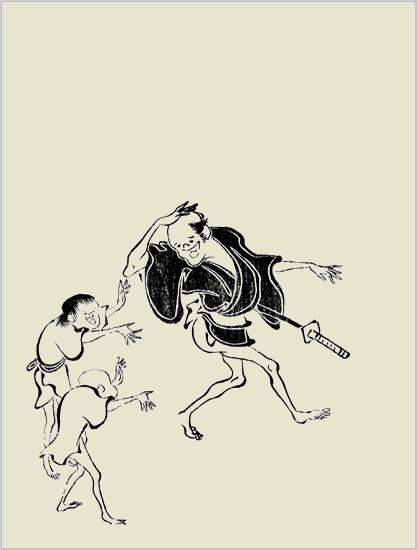
\includegraphics[width=\textwidth]{anthology-13}
\end{figure}

\begin{haiku}
    {\FH おさな子や花を見せても口を明く}\hfill{\FH 星布女}

    \vin{} The tiny child---
    \vin{} \vin{} shown even a flower
    \vin{} \vin{} \vin{} opens its mouth \hspace{\fill} SEIFU-JO
\end{haiku}

\begin{haiku}
    {\FH 蚤の跡かぞへながらに添乳哉}\hfill{\FH 一茶}

    \vin{} Flea bites---
    \vin{} \vin{} while counting them, she nurses
    \vin{} \vin{} \vin{} her baby \hspace{\fill} ISSA
\end{haiku}

\begin{haiku}
    {\FH \ruby{乳呑}{ちのみ}子の風よけに立かがし哉}\hfill{\FH 一茶}

    \vin{} Shielding an infant
    \vin{} \vin{} from the wind---
    \vin{} \vin{} \vin{} a scarecrow \hspace{\fill} ISSA
\end{haiku}

\begin{haiku}
    {\FH 蝶とぶや児這ひつけばつけば又}\hfill{\FH 一茶}

    \vin{} Garden butterfly---
    \vin{} \vin{} as the baby crawls, it flies
    \vin{} \vin{} \vin{} crawls---flies--- \hspace{\fill} ISSA
\end{haiku}

\begin{haiku}
    {\FH 負ふた子に\ruby{蕨}{わらび}をりては持せける}\hfill{\FH 暁台}

    \vin{} A child on my back
    \vin{} \vin{} I picked a bracken shoot
    \vin{} \vin{} \vin{} and let him hold it \hspace{\fill} KY\={O}TAI
\end{haiku}

\begin{haiku}
    {\FH 渋い所母が喰けり山の柿}\hfill{\FH 一茶}

    \vin{} Her mother eats
    \vin{} \vin{} the bitter parts---
    \vin{} \vin{} \vin{} mountain persimmons \hspace{\fill} ISSA
\end{haiku}

\begin{haiku}
    {\FH 名月を取ってくれろと泣く子哉}\hfill{\FH 一茶}

    \vin{} The harvest moon---
    \vin{} \vin{} ``Get it for me!''
    \vin{} \vin{} \vin{} cries the child \hspace{\fill} ISSA
\end{haiku}

\begin{haiku}
    {\FH 是程のぼたんと仕かたする子哉}\hfill{\FH 一茶}

    \vin{} ``It's this big!''
    \vin{} \vin{} forming a peony with her arms---
    \vin{} \vin{} \vin{} a child \hspace{\fill} ISSA
\end{haiku}

\begin{haiku}
    {\FH けふもけふも凧引かかる榎哉}\hfill{\FH 一茶}

    \vin{} Today too!
    \vin{} \vin{} today too! kites caught
    \vin{} \vin{} \vin{} by the nettle tree \hspace{\fill} ISSA
\end{haiku}

\begin{haiku}
    {\FH 春雨や猫におどりをおしえる子}\hfill{\FH 一茶}

    \vin{} Spring rains---
    \vin{} \vin{} a child teaches the cat
    \vin{} \vin{} \vin{} a dance \hspace{\fill} ISSA
\end{haiku}

\begin{haiku}
    NOT FOUND\hfill{\FH 無名氏}

    \vin{} Worse than tears---
    \vin{} \vin{} the smile of the
    \vin{} \vin{} \vin{} abandoned child \hspace{\fill} ANONYMOUS
\end{haiku}

\begin{haiku}
    {\FH 初瓜を引とらまへて寝た子哉}\hfill{\FH 一茶}

    \vin{} The season's first melon
    \vin{} \vin{} clutched in its arms
    \vin{} \vin{} \vin{} sleeps the child \hspace{\fill} ISSA
\end{haiku}

\begin{haiku}
   {\FH 炎天や誰が子はだしの放し飼}\hfill{紅葉}

    \vin{} Blazing sun---
    \vin{} \vin{} whose barefoot child
    \vin{} \vin{} \vin{} is running free? \hspace{\fill} K\={O}Y\={O}
\end{haiku}

\begin{haiku}
   NOT FOUND\hfill{---}

    \vin{} At the ticket window
    \vin{} \vin{} our child becomes
    \vin{} \vin{} \vin{} one year younger \hspace{\fill} SEIUN
\end{haiku}

\begin{haiku}
    {\FH \ruby{末}{すえ}の子や御墓参りの箒持}\hfill{\FH 一茶}

    \vin{} The youngest child
    \vin{} \vin{} visiting family graves
    \vin{} \vin{} \vin{} carries the broom \hspace{\fill} ISSA
\end{haiku}

\begin{haiku}
    {\FH 初恋や燈籠によする顔と顔}\hfill{\FH 太祇}

    \vin{} First love---
    \vin{} \vin{} coming close to a lantern
    \vin{} \vin{} \vin{} face-to-face \hspace{\fill} TAIGI
\end{haiku}

\begin{haiku}
    NOT FOUND\hfill{\FH 無名氏}

    \vin{} Secret night rendezvous---
    \vin{} \vin{} a mosquito was swatted
    \vin{} \vin{} \vin{} and died quietly \hspace{\fill} ANONYMOUS
\end{haiku}

\begin{haiku}
    NOT FOUND\hfill{\FH 而笑子}

    \vin{} Heaven knows,
    \vin{} \vin{} earth knows, every neighbor knows---
    \vin{} \vin{} \vin{} parents don't know \hspace{\fill} JISH\={O}SHI
\end{haiku}

\begin{haiku}
   NOT FOUND\hfill{---}

    \vin{} Sharing one umbrella---
    \vin{} \vin{} the person more in love
    \vin{} \vin{} \vin{} gets wet \hspace{\fill} KEISANJIN
\end{haiku}

\begin{haiku}
    NOT FOUND\hfill{\FH 無名氏}

    \vin{} Catching up
    \vin{} \vin{} and looking at her---
    \vin{} \vin{} \vin{} nothing special \hspace{\fill} ANONYMOUS
\end{haiku}

\begin{haiku}
    NOT FOUND\hfill{\FH 無名氏}

    \vin{} Hearing footsteps
    \vin{} \vin{} splitting in two
    \vin{} \vin{} \vin{} the shadow \hspace{\fill} ANONYMOUS
\end{haiku}

\begin{haiku}
    {\FH 笠でするさらばさらばや薄がすみ}\hfill{\FH 一茶}

    \vin{} Waving umbrellas
    \vin{} \vin{} ``goodbye''\ldots``goodbye''\ldots
    \vin{} \vin{} \vin{} gossamer haze \hspace{\fill} ISSA
\end{haiku}

\begin{haiku}
    NOT FOUND\hfill{\FH 無名氏}

    \vin{} Having children,
    \vin{} \vin{} you understand---
    \vin{} \vin{} \vin{} but too late \hspace{\fill} ANONYMOUS
\end{haiku}

\begin{figure}
    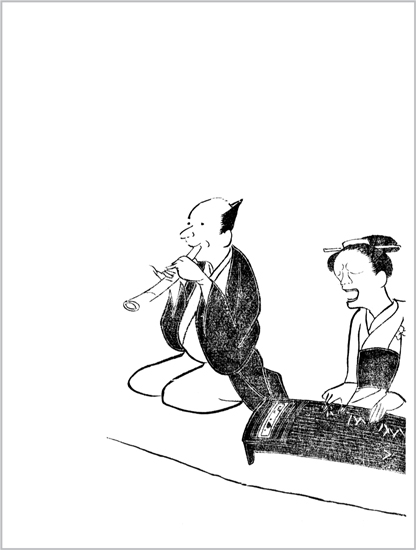
\includegraphics[width=\textwidth]{anthology-14}
\end{figure}

\begin{haiku}
    {\FH 梨の花月に\ruby{書}{ふ}ミよむ女あり}\hfill{\FH 蕪村}

    \vin{} Pear blossoms---
    \vin{} \vin{} a woman reads a letter
    \vin{} \vin{} \vin{} by moonlight \hspace{\fill} BUSON
\end{haiku}

\begin{haiku}
    {\FH 大根引大根で道を教へけり}\hfill{\FH 一茶}

    \vin{} Harvesting radishes,
    \vin{} \vin{} he points the way
    \vin{} \vin{} \vin{} with a radish \hspace{\fill} ISSA
\end{haiku}

\begin{haiku}
   NOT FOUND\hfill{---}

    \vin{} Workers---
    \vin{} \vin{} they laugh
    \vin{} \vin{} \vin{} in a single color \hspace{\fill} HAKUSHI
\end{haiku}

\begin{haiku}
    NOT FOUND\hfill{\FH 無名氏}

    \vin{} Selling ladles,
    \vin{} \vin{} he shows how to scoop up
    \vin{} \vin{} \vin{} nothing at all \hspace{\fill} ANONYMOUS
\end{haiku}

\begin{haiku}
    {法華経の唇ばかり忙しき}\hfill{\FH 無名氏}

    \vin{} Chanting the Lotus Sutra---
    \vin{} \vin{} only his lips
    \vin{} \vin{} \vin{} are busy \hspace{\fill} ANONYMOUS
\end{haiku}

\begin{haiku}
    NOT FOUND\hfill{\FH 無名氏}

    \vin{} With both hands
    \vin{} \vin{} thrust up mightily---
    \vin{} \vin{} \vin{} my yawn \hspace{\fill} ANONYMOUS
\end{haiku}

\begin{haiku}
   NOT FOUND\hfill{---}

    \vin{} Trout fishing---
    \vin{} \vin{} more fishermen
    \vin{} \vin{} \vin{} than trout \hspace{\fill} KENJIN
\end{haiku}

\begin{haiku}
    NOT FOUND\hfill{\FH 無名氏}

    \vin{} Very secretly
    \vin{} \vin{} the medicine peddler
    \vin{} \vin{} \vin{} is sick \hspace{\fill} ANONYMOUS
\end{haiku}

\begin{haiku}
    NOT FOUND\hfill{\FH 無名氏}

    \vin{} The convalescent---
    \vin{} \vin{} indulging in his mother's care
    \vin{} \vin{} \vin{} has become a habit \hspace{\fill} ANONYMOUS
\end{haiku}

\begin{haiku}
    NOT FOUND\hfill{\FH 無名氏}

    \vin{} Losing,
    \vin{} \vin{} he straightens in his seat
    \vin{} \vin{} \vin{} and loses again \hspace{\fill} ANONYMOUS
\end{haiku}

\begin{haiku}
   NOT FOUND\hfill{---}

    \vin{} Having given my opinion
    \vin{} \vin{} I return home to
    \vin{} \vin{} \vin{} my wife's opinion \hspace{\fill} YACH\={O}
\end{haiku}

\begin{haiku}
    NOT FOUND\hfill{\FH 無名氏}

    \vin{} Priding himself
    \vin{} \vin{} on scolding
    \vin{} \vin{} \vin{} his beautiful wife \hspace{\fill} ANONYMOUS
\end{haiku}

\begin{figure}
    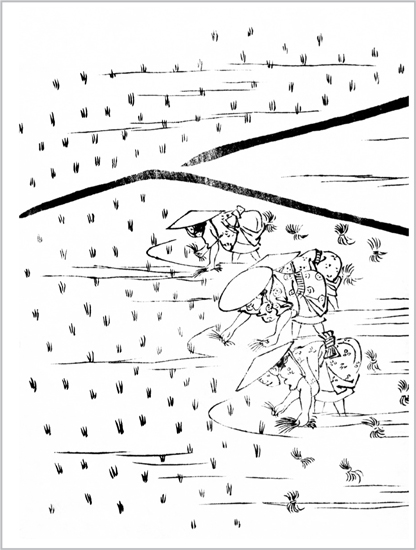
\includegraphics[width=\textwidth]{anthology-15}
\end{figure}

\begin{haiku}
    NOT FOUND\hfill{\FH 無名氏}

    \vin{} ``Every woman\ldots''
    \vin{} \vin{} he starts to say,
    \vin{} \vin{} \vin{} then looks around \hspace{\fill} ANONYMOUS
\end{haiku}

\begin{haiku}
    NOT FOUND\hfill{\FH 無名氏}

    \vin{} ``After you die
    \vin{} \vin{} they'll be valuable''
    \vin{} \vin{} \vin{} he tells the painter \hspace{\fill} ANONYMOUS
\end{haiku}

\begin{haiku}
    {\FH \ruby{骸骨}{がいこつ}の上を\ruby{装}{よそ}ふて花見かな}\hfill{\FH 鬼貫}

    \vin{} Skeletons
    \vin{} \vin{} covered with adornment---
    \vin{} \vin{} \vin{} flower viewing \hspace{\fill} ONITSURA
\end{haiku}

\begin{haiku}
   NOT FOUND\hfill{---}

    \vin{} Wanting to be logical
    \vin{} \vin{} he tries so hard---
    \vin{} \vin{} \vin{} the drunkard \hspace{\fill} MEITEI
\end{haiku}

\begin{haiku}
    NOT FOUND\hfill{\FH 無名氏}

    \vin{} ``Let's pull them all''
    \vin{} \vin{} says the dentist
    \vin{} \vin{} \vin{} generously \hspace{\fill} ANONYMOUS
\end{haiku}

\begin{haiku}
    {\FH 負まじき角力を寝ものがたり哉}\hfill{\FH 蕪村}

    \vin{} ``I'd never lose
    \vin{} \vin{} in a sumo match''---
    \vin{} \vin{} \vin{} pillow talk \hspace{\fill} BUSON
\end{haiku}

\begin{haiku}
    {\FH のふなしはつみも又なし冬ごもり}\hfill{\FH 一茶}

    \vin{} No talents
    \vin{} \vin{} also no sins---
    \vin{} \vin{} \vin{} winter seclusion \hspace{\fill} ISSA
\end{haiku}

\begin{haiku}
    {\FH 冬ごもり妻にも子にもかくれん坊}\hfill{\FH 蕪村}

    \vin{} Winter seclusion---
    \vin{} \vin{} from my wife and children
    \vin{} \vin{} \vin{} I too play hide-and-seek \hspace{\fill} BUSON
\end{haiku}

\begin{haiku}
   NOT FOUND\hfill{---}

    \vin{} New Year's cards
    \vin{} \vin{} with women's handwriting
    \vin{} \vin{} \vin{} get looked at first \hspace{\fill} BIRIKEN
\end{haiku}

\begin{haiku}
    {口聞かぬ膝へ口きく膝を乗せ}\hfill{\FH 無名氏}

    \vin{} She lowers
    \vin{} \vin{} her eloquent lap
    \vin{} \vin{} \vin{} onto his silent lap \hspace{\fill} ANONYMOUS
\end{haiku}

\begin{haiku}
    {\FH \ruby{花衣}{はなごろも}ぬぐやまつはる紐{ひも}いろいろ}\hfill{\FH 久女}

    \vin{} The kimono for flower-viewing---
    \vin{} \vin{} disrobing, I'm entwined in
    \vin{} \vin{} \vin{} a myriad of sashes \hspace{\fill} HISA-JO
\end{haiku}

\begin{haiku}
    {\FH 物言わず客と亭主と白菊と}\hfill{\FH 蓼太}

    \vin{} Without a word
    \vin{} \vin{} the guest, the host,
    \vin{} \vin{} \vin{} white chrysanthemums \hspace{\fill} RY\={O}TA
\end{haiku}

\begin{haiku}
    {\FH 門を\ruby{出}{いず}ればわれも行人秋のくれ}\hfill{\FH 蕪村}

    \vin{} Out from the gate,
    \vin{} \vin{} I too become a traveler---
    \vin{} \vin{} \vin{} autumn dusk \hspace{\fill} BUSON
\end{haiku}

\begin{haiku}
    {\FH 川に沿ふて行けど橋なし日の永き}\hfill{\FH 子規}

    \vin{} Walking along the river
    \vin{} \vin{} with no bridge to cross---
    \vin{} \vin{} \vin{} the day is long \hspace{\fill} SHIKI
\end{haiku}

\begin{haiku}
    {\FH 寒月や小石のさはる\ruby{沓}{くつ}の底}\hfill{\FH 蕪村}

    \vin{} Cold moon---
    \vin{} \vin{} feeling the pebbles
    \vin{} \vin{} \vin{} under my shoes \hspace{\fill} BUSON
\end{haiku}

\begin{haiku}
    {\FH 一人来て一人を\ruby{訪}{と}ふや秋のくれ}\hfill{\FH 蕪村}

    \vin{} A single guest
    \vin{} \vin{} visits a single host---
    \vin{} \vin{} \vin{} autumn evening \hspace{\fill} BUSON
\end{haiku}

\begin{haiku}
    {\FH 応々と言へど\ruby{叩}{たた}くや雪の門}\hfill{\FH 去来}

    \vin{} ``Coming, coming'',
    \vin{} \vin{} but someone still knocks---
    \vin{} \vin{} \vin{} snowy gate \hspace{\fill} KYORAI
\end{haiku}

\begin{figure}
    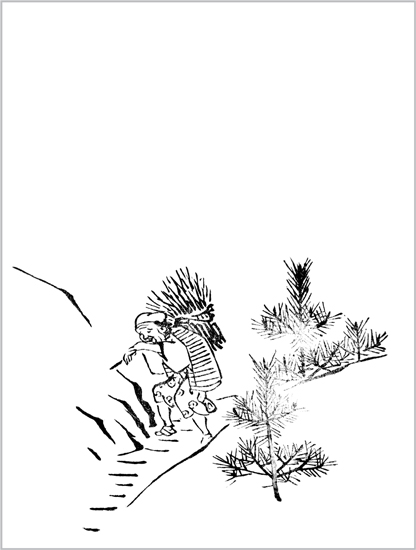
\includegraphics[width=\textwidth]{anthology-16}
\end{figure}

\begin{haiku}
    NOT FOUND\hfill{\FH 無名氏}

    \vin{} My go rival---
    \vin{} \vin{} how vexing
    \vin{} \vin{} \vin{} and how dear \hspace{\fill} ANONYMOUS
\end{haiku}

\begin{haiku}
    NOT FOUND\hfill{\FH 宗長}

    \vin{} Getting old---
    \vin{} \vin{} I slip on a watermelon rind
    \vin{} \vin{} \vin{} as I dance \hspace{\fill} S\={O}CH\={O}
\end{haiku}

\begin{haiku}
    {\FH はなたれて独り碁をうつ夜寒かな}\hfill{\FH 蕪村}

    \vin{} My nose running
    \vin{} \vin{} I play a solitary go-game---
    \vin{} \vin{} \vin{} night chill \hspace{\fill} BUSON
\end{haiku}

\begin{haiku}
   NOT FOUND\hfill{---}

    \vin{} Just asking them to fight,
    \vin{} \vin{} he saved tons of money
    \vin{} \vin{} \vin{} and died \hspace{\fill} HAKUCH\={O}
\end{haiku}

\begin{haiku}
    {\FH 肉がやせてくる太い骨である}\hfill{\FH 放哉}

    \vin{} Flesh getting thin---
    \vin{} \vin{} these are thick bones \hspace{\fill} H\={O}SAI
\end{haiku}

\begin{haiku}
    {\FH 我骨のふとんにさはる霜夜哉}\hfill{\FH 蕪村}

    \vin{} Feeling my bones
    \vin{} \vin{} on the quilting---
    \vin{} \vin{} \vin{} frosty night \hspace{\fill} BUSON
\end{haiku}

\begin{haiku}
    {\FH \ruby{炭}{すみ}の火や\ruby{齢}{よわい}のへるもあの通り}\hfill{\FH 一茶}

    \vin{} Charcoal fire---
    \vin{} \vin{} my years dwindle down
    \vin{} \vin{} \vin{} just like that \hspace{\fill} ISSA
\end{haiku}

\begin{haiku}
    {\FH 行く我にとどまる汝に秋二つ}\hfill{\FH 子規}

    \vin{} For me leaving
    \vin{} \vin{} for you staying
    \vin{} \vin{} \vin{} two autumns \hspace{\fill} SHIKI
\end{haiku}

\begin{haiku}
    {\FH 何もないが心安さよ涼しさよ}\hfill{\FH 一茶}

    \vin{} Owning nothing---
    \vin{} \vin{} such peace,
    \vin{} \vin{} \vin{} such coolness! \hspace{\fill} ISSA
\end{haiku}

\begin{haiku}
    {\FH 生残り生残りたる寒かな}\hfill{\FH 一茶}

    \vin{} Left to live on
    \vin{} \vin{} left to live on and on---
    \vin{} \vin{} \vin{} this cold \hspace{\fill} ISSA
\end{haiku}

\begin{haiku}
    {\FH さびしさのうれしくもあり秋の暮}\hfill{\FH 蕪村}

    \vin{} Loneliness
    \vin{} \vin{} also has its pleasure---
    \vin{} \vin{} \vin{} autumn dusk \hspace{\fill} BUSON
\end{haiku}

\begin{haiku}
    {\FH 身の秋や月は無きずの月ながら}\hfill{\FH 一茶}

    \vin{} Autumn of my years---
    \vin{} \vin{} the moon is perfect
    \vin{} \vin{} \vin{} and yet--- \hspace{\fill} ISSA
\end{haiku}

\begin{haiku}
   NOT FOUND\hfill{---}

    \vin{} Walking the dog
    \vin{} \vin{} you meet
    \vin{} \vin{} \vin{} lots of dogs \hspace{\fill} S\={O}SHI
\end{haiku}

\begin{haiku}
    {\FH \ruby{居眠}{いねぶ}りて我にかくれん冬ごもり}\hfill{\FH 蕪村}

    \vin{} Taking a nap
    \vin{} \vin{} I hide within myself---
    \vin{} \vin{} \vin{} winter seclusion \hspace{\fill} BUSON
\end{haiku}

\begin{haiku}
    {\FH がつくりと抜け\ruby{初}{そめ}る歯や秋の風}\hfill{\FH 杉風}

    \vin{} All of a sudden
    \vin{} \vin{} my first fallen tooth---
    \vin{} \vin{} \vin{} autumn wind \hspace{\fill} SANP\={U}
\end{haiku}

\begin{haiku}
    {\FH しぐるるや死なないでいる}\hfill{\FH 山頭火}

    \vin{} Winter rain---
    \vin{} \vin{} I'm not dead yet \hspace{\fill} SANT\={O}KA
\end{haiku}

\begin{haiku}
    {\FH 家はみな杖に\ruby{白髪}{しらが}の墓参り}\hfill{\FH 芭蕉}

    \vin{} A whole family
    \vin{} \vin{} all gray-haired with canes
    \vin{} \vin{} \vin{} visits graves \hspace{\fill} BASH\={O}
\end{haiku}

\begin{haiku}
    {\FH この秋はひざに子のない月見かな}\hfill{\FH 鬼貫}

    \vin{} This autumn
    \vin{} \vin{} no child in my lap---
    \vin{} \vin{} \vin{} moon-viewing \hspace{\fill} ONITSURA
\end{haiku}

\begin{haiku}
    NOT FOUND\hfill{\FH 無名氏}

    \vin{} Are my youthful dreams
    \vin{} \vin{} still unfinished?
    \vin{} \vin{} \vin{} this morning's frost \hspace{\fill} ANONYMOUS
\end{haiku}

\begin{haiku}
    {\FH \ruby{目出度}{めでた}さも\ruby{中}{ちう}\ruby{位也}{くらい}おらが春}\hfill{\FH 一茶}

    \vin{} The auspiciousness
    \vin{} \vin{} is just about medium---
    \vin{} \vin{} \vin{} my spring \hspace{\fill} ISSA
\end{haiku}

\begin{haiku}
    NOT FOUND\hfill{\FH 無名氏}

    \vin{} On New Year's Day
    \vin{} \vin{} the morning in town
    \vin{} \vin{} \vin{} comes irregularly \hspace{\fill} ANONYMOUS
\end{haiku}

\begin{haiku}
    {\FH 早立のかぶせてくれし衾哉}\hfill{\FH 一茶}

    \vin{} First winter kimono---
    \vin{} \vin{} may you quickly grow to
    \vin{} \vin{} \vin{} a naughty age \hspace{\fill} ISSA
\end{haiku}

\begin{haiku}
    {\FH 雪とけて村一ぱいの子ども哉}\hfill{\FH 一茶}

    \vin{} Snow has melted---
    \vin{} \vin{} the village is full
    \vin{} \vin{} \vin{} of children \hspace{\fill} ISSA
\end{haiku}

\chapter{Resonance and Reverberation}

\begin{figure}
    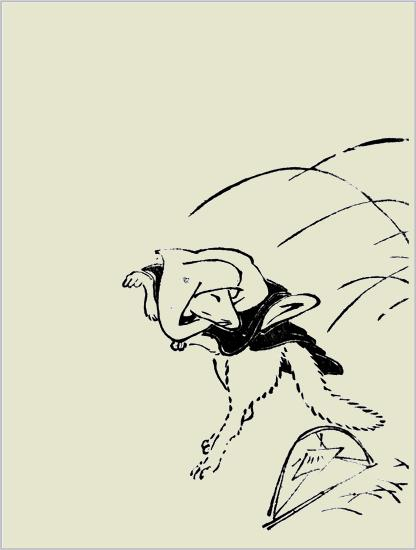
\includegraphics[width=\textwidth]{anthology-17}
\end{figure}

\begin{haiku}
    {\FH な折りそと折りてくれけり園の梅}\hfill{\FH 太祇}

    \vin{} ``Don't dare break it!''
    \vin{} \vin{} but he broke off and gave me
    \vin{} \vin{} \vin{} a branch of garden plum \hspace{\fill} TAIGI
\end{haiku}

\begin{haiku}
    NOT FOUND\hfill{\FH 把栗}

    \vin{} Spring river---
    \vin{} \vin{} a tiny wooden clog
    \vin{} \vin{} \vin{} floats by \hspace{\fill} HARITSU
\end{haiku}

\begin{haiku}
    {\FH 春雨や薮に吹るる捨手紙}\hfill{\FH 一茶}

    \vin{} Spring rain---
    \vin{} \vin{} blown onto the bush
    \vin{} \vin{} \vin{} a discarded letter \hspace{\fill} ISSA
\end{haiku}

\begin{haiku}
    {\FH 摘むもをしつまぬもをしき菫かな}\hfill{\FH 直女}

    \vin{} A shame to pick it
    \vin{} \vin{} a shame to leave it---
    \vin{} \vin{} \vin{} the violet \hspace{\fill} NAO-JO
\end{haiku}

\begin{haiku}
    {\FH 追はれても急がぬふりの蝶々哉}\hfill{\FH 我樂}

    \vin{} Even when chased
    \vin{} \vin{} it pretends not to hurry---
    \vin{} \vin{} \vin{} the butterfly \hspace{\fill} GARAKU
\end{haiku}

\begin{haiku}
    {\FH くさめして見失うたる雲雀かな}\hfill{\FH 也有}

    \vin{} One sneeze---
    \vin{} \vin{} and I lost sight of
    \vin{} \vin{} \vin{} the skylark \hspace{\fill} YAY\={U}
\end{haiku}

\begin{haiku}
    {\FH こころ疲れて山が海が美しすぎる}\hfill{\FH 山頭火}

    \vin{} Tired heart---
    \vin{} \vin{} mountains and ocean
    \vin{} \vin{} \vin{} too much beauty \hspace{\fill} SANT\={O}KA
\end{haiku}

\begin{haiku}
    NOT FOUND\hfill{\FH 曰人}

    \vin{} Lead him slowly!
    \vin{} \vin{} the horse is carrying
    \vin{} \vin{} \vin{} the spring moon \hspace{\fill} ATSUJIN
\end{haiku}

\begin{haiku}
    {\FH \ruby{外}{と}にも出よ触るるばかりに春の月}\hfill{\FH 汀女}

    \vin{} Come out!
    \vin{} \vin{} you can almost touch
    \vin{} \vin{} \vin{} the spring moon \hspace{\fill} TEI-JO
\end{haiku}

\begin{haiku}
    {\FH 春の月さはらば雫たりぬべし}\hfill{\FH 一茶}

    \vin{} Spring moon---
    \vin{} \vin{} if I touch it, it would
    \vin{} \vin{} \vin{} drip \hspace{\fill} ISSA
\end{haiku}

\begin{haiku}
    {\FH 春雨や\ruby{欠}{あくび}をうつる門の犬}\hfill{\FH 一茶}

    \vin{} Spring rain---
    \vin{} \vin{} I gave my yawn
    \vin{} \vin{} \vin{} to the dog at the gate \hspace{\fill} ISSA
\end{haiku}

\begin{haiku}
    {もの思う向こうを通るかたつむり}\hfill{\FH 無名氏}

    \vin{} While I ponder
    \vin{} \vin{} a snail
    \vin{} \vin{} \vin{} passes me by \hspace{\fill} ANONYMOUS
\end{haiku}

\begin{haiku}
   NOT FOUND\hfill{---}

    \vin{} Frogs grow silent---
    \vin{} \vin{} noble humans
    \vin{} \vin{} \vin{} are passing by \hspace{\fill} RAKUKYO
\end{haiku}

\begin{haiku}
    NOT FOUND\hfill{\FH 把栗}

    \vin{} Early summer rain---
    \vin{} \vin{} a letter from home
    \vin{} \vin{} \vin{} arrives wet \hspace{\fill} HARITSU
\end{haiku}

\begin{haiku}
    {\FH 夕立や裸で乗しはだか馬}\hfill{\FH 一茶}

    \vin{} Sudden shower---
    \vin{} \vin{} riding naked
    \vin{} \vin{} \vin{} on a naked horse \hspace{\fill} ISSA
\end{haiku}

\begin{haiku}
    {\FH 石も木も\ruby{眼}{まなこ}に光る暑さかな}\hfill{\FH 去来}

    \vin{} Rocks and trees
    \vin{} \vin{} glisten in my eyes---
    \vin{} \vin{} \vin{} such heat \hspace{\fill} KYORAI
\end{haiku}

\begin{haiku}
    {\FH 石工の鑿冷したる清水かな}\hfill{\FH 蕪村}

    \vin{} The stone-carver
    \vin{} \vin{} cools his chisel
    \vin{} \vin{} \vin{} in the clear stream \hspace{\fill} BUSON
\end{haiku}

\begin{haiku}
    {\FH \ruby{鍬}{くわ}立てゝあたり人なき熱さ哉}\hfill{\FH 子規}

    \vin{} A hoe standing
    \vin{} \vin{} with no one around---
    \vin{} \vin{} \vin{} the heat! \hspace{\fill} SHIKI
\end{haiku}

\begin{figure}
    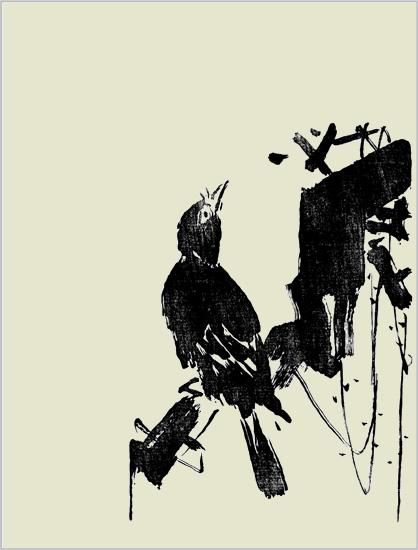
\includegraphics[width=\textwidth]{anthology-18}
\end{figure}

\begin{haiku}
    {\FH 牛に成る合点ぞ\ruby{朝寐}{あさね}夕すゞみ}\hfill{\FH 支考}

    \vin{} Becoming a cow
    \vin{} \vin{} would be fine---morning naps
    \vin{} \vin{} \vin{} and the evening cool \hspace{\fill} SHIK\={O}
\end{haiku}

\begin{haiku}
    NOT FOUND\hfill{\FH 野水}

    \vin{} After my sneeze
    \vin{} \vin{} all is quiet---
    \vin{} \vin{} \vin{} summer mountains \hspace{\fill} YASUI
\end{haiku}

\begin{haiku}
    {\FH 月と我ばかり残りぬ橋涼み}\hfill{\FH 菊舎}

    \vin{} Only the moon and I
    \vin{} \vin{} remain on the bridge
    \vin{} \vin{} \vin{} cooling off \hspace{\fill} KIKUSHA
\end{haiku}

\begin{haiku}
    {\FH 人一人蝿も一つや大座敷}\hfill{\FH 一茶}

    \vin{} One person
    \vin{} \vin{} and one fly
    \vin{} \vin{} \vin{} in the large room \hspace{\fill} ISSA
\end{haiku}

\begin{haiku}
    {\FH 縁の蝿手をする所を打れけり}\hfill{\FH 一茶}

    \vin{} The fly on the porch
    \vin{} \vin{} while rubbing its hands---
    \vin{} \vin{} \vin{} swat! \hspace{\fill} ISSA
\end{haiku}

\begin{haiku}
    {\FH 蝿一つ打てはなむあみだ仏哉}\hfill{\FH 一茶}

    \vin{} Each time
    \vin{} \vin{} I swat a fly, I chant
    \vin{} \vin{} \vin{} ``Namu Amida Butsu'' \hspace{\fill} ISSA
\end{haiku}

\begin{haiku}
    {\FH ぼうふりも御経の\ruby{拍子}{ひょうし}とりにけり}\hfill{\FH 一茶}

    \vin{} Mosquito larvae,
    \vin{} \vin{} dancing a Buddhist chant
    \vin{} \vin{} \vin{} in the water by the grave \hspace{\fill} ISSA
\end{haiku}

\begin{haiku}
    {\FH 叩かれて昼の蚊を吐く木魚哉}\hfill{\FH 漱石}

    \vin{} Being hit
    \vin{} \vin{} the gong spits out
    \vin{} \vin{} \vin{} a noontime mosquito \hspace{\fill} S\={O}SEKI
\end{haiku}

\begin{haiku}
    {\FH 血を分けし身とは思はず蚊の憎き}\hfill{\FH 丈草}

    \vin{} Sharing the same blood
    \vin{} \vin{} but we're not related---
    \vin{} \vin{} \vin{} the hateful mosquito! \hspace{\fill} J\={O}S\={O}
\end{haiku}

\begin{haiku}
    NOT FOUND\hfill{\FH 許六}

    \vin{} The flute player
    \vin{} \vin{} bitten by a mosquito
    \vin{} \vin{} \vin{} on the edge of his lips \hspace{\fill} KYOROKU
\end{haiku}

\begin{haiku}
    {\FH 蚊柱や是もなければ小淋しき}\hfill{\FH 一茶}

    \vin{} Swarms of mosquitoes---
    \vin{} \vin{} but without them,
    \vin{} \vin{} \vin{} it's a little lonely \hspace{\fill} ISSA
\end{haiku}

\begin{haiku}
    {\FH 昼の蚊を後ろにかくす仏かな}\hfill{\FH 一茶}

    \vin{} During the day
    \vin{} \vin{} the Buddha shelters behind
    \vin{} \vin{} \vin{} mosquitoes \hspace{\fill} ISSA
\end{haiku}

\begin{figure}
    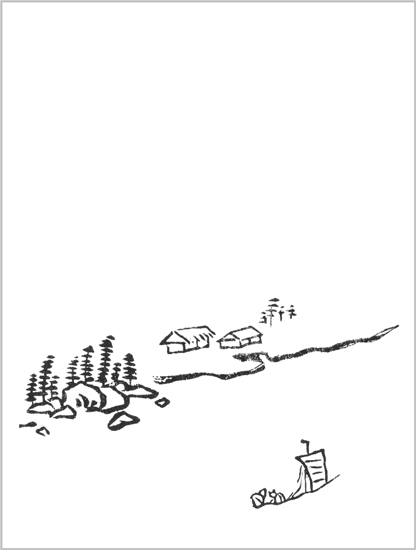
\includegraphics[width=\textwidth]{anthology-19}
\end{figure}

\begin{haiku}
    {\FH 乞食かな天地を着たる夏衣}\hfill{\FH 其角}

    \vin{} The beggar
    \vin{} \vin{} wears heaven and earth
    \vin{} \vin{} \vin{} as summer clothes \hspace{\fill} KIKAKU
\end{haiku}

\begin{haiku}
    {\FH 人有れば蝿あり仏ありにけり}\hfill{\FH 一茶}

    \vin{} Where there are people
    \vin{} \vin{} there are flies, and
    \vin{} \vin{} \vin{} there are Buddhas \hspace{\fill} ISSA
\end{haiku}

\begin{haiku}
    {\FH 長生の蝿よ蚤蚊よ貧乏村}\hfill{\FH 一茶}

    \vin{} They live long---
    \vin{} \vin{} the flies, fleas, and mosquitoes
    \vin{} \vin{} \vin{} in this poor village \hspace{\fill} ISSA
\end{haiku}

\begin{haiku}
    NOT FOUND\hfill{\FH 無名氏}

    \vin{} Two old bent backs
    \vin{} \vin{} sitting close, wrapped in
    \vin{} \vin{} \vin{} a shower of cicada songs \hspace{\fill} ANONYMOUS
\end{haiku}

\begin{haiku}
    {\FH 手のうへにかなしく消る蛍かな}\hfill{\FH 去来}

    \vin{} In my hand
    \vin{} \vin{} its fleeting light vanishes---
    \vin{} \vin{} \vin{} the firefly \hspace{\fill} KYORAI
\end{haiku}

\begin{haiku}
    NOT FOUND\hfill{\FH 把栗}

    \vin{} How delightful
    \vin{} \vin{} walking on dewy grasses---
    \vin{} \vin{} \vin{} straw sandals \hspace{\fill} HARITSU
\end{haiku}

\begin{haiku}
    {\FH 蜘殺すあとの淋しき夜寒哉}\hfill{\FH 子規}

    \vin{} Killing the spider
    \vin{} \vin{} then so lonesome---
    \vin{} \vin{} \vin{} evening cold \hspace{\fill} SHIKI
\end{haiku}

\begin{haiku}
    {\FH 年寄と見るや鳴蚊も耳の際}\hfill{\FH 一茶}

    \vin{} Seeing that I'm old
    \vin{} \vin{} even the mosquito whispers
    \vin{} \vin{} \vin{} closer to my ear \hspace{\fill} ISSA
\end{haiku}

\begin{haiku}
    {\FH 秋の蚊や死ぬる覺期でわれを刺す}\hfill{\FH 子規}

    \vin{} An autumn mosquito
    \vin{} \vin{} determined to die
    \vin{} \vin{} \vin{} bites me \hspace{\fill} SHIKI
\end{haiku}

\begin{haiku}
    {\FH 白菊にしばしたゆたふはさみかな}\hfill{\FH 蕪村}

    \vin{} Before the white chrysanthemums
    \vin{} \vin{} hesitating for a while---
    \vin{} \vin{} \vin{} the scissors \hspace{\fill} BUSON
\end{haiku}

\begin{haiku}
    {\FH 秋来ぬと合点させたる\ruby{嚔}{くしゃみ}かな}\hfill{\FH 蕪村}

    \vin{} Truly the autumn has come---
    \vin{} \vin{} I was convinced
    \vin{} \vin{} \vin{} by my sneeze \hspace{\fill} BUSON
\end{haiku}

\begin{haiku}
    NOT FOUND\hfill{\FH 把栗}

    \vin{} Planting my buttocks
    \vin{} \vin{} on a huge taro leaf---
    \vin{} \vin{} \vin{} moon-viewing \hspace{\fill} HARITSU
\end{haiku}

\begin{haiku}
    {\FH 何着てもうつくしうなる月見かな}\hfill{\FH 千代女}

    \vin{} Whatever they wear
    \vin{} \vin{} they become beautiful
    \vin{} \vin{} \vin{} moon-viewing \hspace{\fill} CHIYO-JO
\end{haiku}

\begin{figure}
    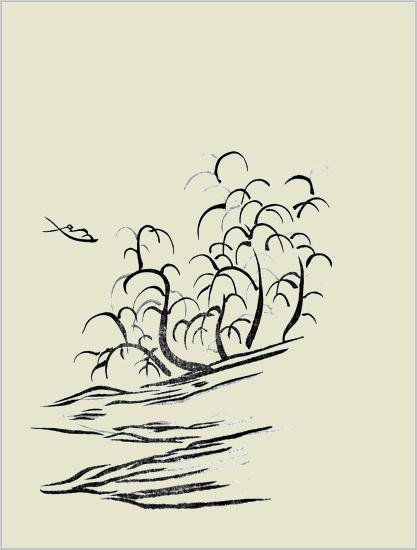
\includegraphics[width=\textwidth]{anthology-20}
\end{figure}

\begin{haiku}
    {\FH われをつれて我影帰る月見かな}\hfill{\FH 素堂}

    \vin{} Taking me along
    \vin{} \vin{} my shadow comes home
    \vin{} \vin{} \vin{} from moon-viewing \hspace{\fill} SOD\={O}
\end{haiku}

\begin{haiku}
    {\FH 婆々どのが酒呑に行く月よ哉}\hfill{\FH 一茶}

    \vin{} Even grandma
    \vin{} \vin{} goes out drinking---
    \vin{} \vin{} \vin{} moonlit night \hspace{\fill} ISSA
\end{haiku}

\begin{haiku}
    {\FH 雁わやわやおれが噂を\ruby{致}{いた}す哉}\hfill{\FH 一茶}

    \vin{} Wild geese muttering, muttering---
    \vin{} \vin{} are they spreading
    \vin{} \vin{} \vin{} rumors about me? \hspace{\fill} ISSA
\end{haiku}

\begin{haiku}
    {\FH 鳴な雁どつこも同じうき世ぞや}\hfill{\FH 一茶}

    \vin{} Don't cry, wild geese,
    \vin{} \vin{} it's the same everywhere---
    \vin{} \vin{} \vin{} this floating world \hspace{\fill} ISSA
\end{haiku}

\begin{haiku}
    NOT FOUND\hfill{\FH 無名氏}

    \vin{} A man raking---
    \vin{} \vin{} the leaves keep
    \vin{} \vin{} \vin{} calling him back \hspace{\fill} ANONYMOUS
\end{haiku}

\begin{haiku}
    {\FH 夕暮や土とかたればちる木の葉}\hfill{\FH 一茶}

    \vin{} Dusk---
    \vin{} \vin{} while the earth and I talk
    \vin{} \vin{} \vin{} leaves fall \hspace{\fill} ISSA
\end{haiku}

\begin{haiku}
    {\FH 喜べばしきりに落つる木の実かな}\hfill{\FH 風生}

    \vin{} When I show my delight
    \vin{} \vin{} they fall down faster---
    \vin{} \vin{} \vin{} acorns \hspace{\fill} F\={U}SEI
\end{haiku}

\begin{haiku}
    {\FH \ruby{冷冷}{ひえびえ}と袖に入る日や秋の山}\hfill{\FH 一茶}

    \vin{} Coldly, coldly
    \vin{} \vin{} the sun slips into my sleeve---
    \vin{} \vin{} \vin{} autumn mountains \hspace{\fill} ISSA
\end{haiku}

\begin{haiku}
    {\FH 秋風や心の中の幾山河}\hfill{\FH 虚子}

    \vin{} Autumn wind---
    \vin{} \vin{} in my heart, how many
    \vin{} \vin{} \vin{} mountains and rivers \hspace{\fill} KYOSHI
\end{haiku}

\begin{haiku}
    {\FH 山深し心に落つる秋の水}\hfill{\FH 心敬}

    \vin{} Deep in the mountains---
    \vin{} \vin{} falling into my heart
    \vin{} \vin{} \vin{} autumn streams \hspace{\fill} SHINKEI
\end{haiku}

\begin{haiku}
    {\FH 去年より又さびいしひぞ秋の暮}\hfill{\FH 蕪村}

    \vin{} More than last year
    \vin{} \vin{} it is lonely---
    \vin{} \vin{} \vin{} the autumn dusk \hspace{\fill} BUSON
\end{haiku}

\begin{haiku}
    {\FH 肩に来て人なつかしき赤とんぼ}\hfill{\FH 漱石}

    \vin{} On my shoulder
    \vin{} \vin{} is it longing for a companion?
    \vin{} \vin{} \vin{} a red dragonfly \hspace{\fill} S\={O}SEKI
\end{haiku}

\begin{haiku}
    {\FH 老が恋わすれんとすればしぐれかな}\hfill{\FH 蕪村}

    \vin{} Love in my old age---
    \vin{} \vin{} as I try to forget,
    \vin{} \vin{} \vin{} late autumn rain \hspace{\fill} BUSON
\end{haiku}

\begin{haiku}
    {\FH 死んでしまへば雑草雨ふる}\hfill{\FH 山頭火}

    \vin{} When I finally die---
    \vin{} \vin{} weeds
    \vin{} \vin{} \vin{} falling rain \hspace{\fill} SANT\={O}KA
\end{haiku}

\begin{haiku}
    {\FH 野仏の御鼻の先の氷柱哉}\hfill{\FH 一茶}

    \vin{} From the nose
    \vin{} \vin{} of the Buddha in the fields---
    \vin{} \vin{} \vin{} icicles \hspace{\fill} ISSA
\end{haiku}

\begin{haiku}
    {\FH 来る人が道つくるなり門の雪}\hfill{\FH 一茶}

    \vin{} Visitors
    \vin{} \vin{} kindly create a path
    \vin{} \vin{} \vin{} through the snow at my gate \hspace{\fill} ISSA
\end{haiku}

\begin{haiku}
    {\FH 黒犬を\ruby{提灯}{ちょうちん}にする雪の道}\hfill{\FH 無名氏}

    \vin{} The black dog
    \vin{} \vin{} becomes a lantern---
    \vin{} \vin{} \vin{} snowy road \hspace{\fill} ANONYMOUS
\end{haiku}

\begin{haiku}
    {\FH 冬の日や馬上に凍る影法師}\hfill{\FH 芭蕉}

    \vin{} Winter sun---
    \vin{} \vin{} frozen on horseback
    \vin{} \vin{} \vin{} is my shadow \hspace{\fill} BASH\={O}
\end{haiku}

\begin{haiku}
    {\FH つめたさに箒捨けり松の下}\hfill{\FH 太祇}

    \vin{} Piercing cold---
    \vin{} \vin{} I dropped my broom
    \vin{} \vin{} \vin{} under the pines \hspace{\fill} TAIGI
\end{haiku}

\begin{haiku}
    {\FH 雪よりも寒し白髪に冬の月}\hfill{\FH 丈草}

    \vin{} Colder than snow
    \vin{} \vin{} on my white hair---
    \vin{} \vin{} \vin{} the winter moon \hspace{\fill} J\={O}S\={O}
\end{haiku}

\begin{haiku}
    {\FH 霜百里舟中に我月を領す}\hfill{\FH 蕪村}

    \vin{} A hundred miles of frost---
    \vin{} \vin{} in a boat, I own
    \vin{} \vin{} \vin{} the moon \hspace{\fill} BUSON
\end{haiku}

\begin{haiku}
    {\FH 安か安か寒か寒か雪雪}\hfill{\FH 山頭火}

    \vin{} Peaceful, peaceful
    \vin{} \vin{} chilly, chilly
    \vin{} \vin{} \vin{} snow, snow \hspace{\fill} SANT\={O}KA
\end{haiku}

\begin{haiku}
    {\FH ねこに来る賀状や猫のくすしより}\hfill{\FH より江}

    \vin{} To my cat
    \vin{} \vin{} a New Year's card
    \vin{} \vin{} \vin{} from its vet \hspace{\fill} YORIE
\end{haiku}

\begin{haiku}
    {\FH 膝の児の\ruby{指}{ゆびさし}始梅の花}\hfill{\FH 一茶}

    \vin{} The child on my lap
    \vin{} \vin{} begins to point at
    \vin{} \vin{} \vin{} plum blossoms \hspace{\fill} ISSA
\end{haiku}

\begin{haiku}
    {\FH 梅の花ここを盗めとさす月よ}\hfill{\FH 一茶}

    \vin{} Plum blossoms---
    \vin{} \vin{} ``Steal this one here!''
    \vin{} \vin{} \vin{} points the moon \hspace{\fill} ISSA
\end{haiku}

\begin{haiku}
    {\FH 木のもとに汁も膾も桜かな}\hfill{\FH 芭蕉}

    \vin{} Under the trees
    \vin{} \vin{} into the salad, into the soup---
    \vin{} \vin{} \vin{} cherry blossoms \hspace{\fill} BASH\={O}
\end{haiku}
